% ACM conference template for Overleaf/TeX
% This file is a minimal example. For full options, see the ACM documentation.
\documentclass[sigconf]{acmart}

% Remove the ACM copyright for preprints (optional, comment out for submission)
%\settopmatter{printacmref=false}
%\renewcommand\footnotetextcopyrightpermission[1]{}

% Required packages
\usepackage{graphicx}
\usepackage{subfig}
\usepackage{algorithmic}
\usepackage{xcolor}
\usepackage{comment}
\usepackage{soul}
\usepackage{textcomp}

% Note: hyperref is already included in acmart class, don't load it separately

\AtBeginDocument{%
  \providecommand\BibTeX{{%
    Bib\TeX}}}

\begin{document}

\title{A Multi-Simulation Bridge for IoT Digital Twins}

\author{Marco Picone}
\affiliation{%
  \institution{University of Modena and Reggio Emilia}%
  \country{Italy}%
}
\author{Samuele Burattini}
\affiliation{%
  \institution{University of Bologna}%
  \country{Italy}%
}
\author{Marco Melloni}
\affiliation{%
  \institution{University of Modena and Reggio Emilia}%
  \country{Italy}%
}
\author{Prasad Talasila}
\affiliation{%
  \institution{Aarhus University}%
  \city{Aarhus}%
  \country{Denmark}%
}
\author{Davide Ziglioli}
\affiliation{%
  \institution{University of Modena and Reggio Emilia}%
  \country{Italy}%
}
\author{Matteo Martinelli}
\affiliation{%
  \institution{University of Modena and Reggio Emilia}%
  \country{Italy}%
}
\author{Nicola Bicocchi}
\affiliation{%
  \institution{University of Modena and Reggio Emilia}%
  \country{Italy}%
}
\author{Alessandro Ricci}
\affiliation{%
  \institution{University of Bologna}%
  \country{Italy}%
}
\author{Peter Gorm Larsen}
\affiliation{%
  \institution{Aarhus University}%
  \city{Aarhus}%
  \country{Denmark}%
}
\renewcommand{\shortauthors}{Picone et al.}

\begin{abstract}
The increasing capabilities of Digital Twins (DTs) in the context of the Internet of Things (IoT) and Industrial IoT (IIoT) call for seamless integration with simulation platforms to support system design, validation, and real-time operation. This paper introduces the concept, design, and experimental evaluation of the \emph{DT Simulation Bridge}---a software framework that enables diverse interaction patterns between active DTs and simulation environments.
The framework supports both the DT development lifecycle and the incorporation of simulations during active operation. Through bidirectional data exchange, simulations can update DT models dynamically, while DTs provide real-time feedback to adapt simulation parameters. We describe the architectural design and core software components that ensure flexible interoperability and scalable deployment.
Experimental results show that the DT Simulation Bridge enhances design agility, facilitates virtual commissioning, and supports live behavioral analysis under realistic conditions, demonstrating its effectiveness across a range of industrial scenarios.
\end{abstract}

\keywords{Digital Twins, Industry, Simulation Bridge, Simulators, Agents}

% CCS concepts (mandatory for papers over two pages)
\begin{CCSXML}
<ccs2012>
   <concept>
       <concept_id>10010147.10010178.10010205.10010208</concept_id>
       <concept_desc>Computing methodologies~Distributed simulation</concept_desc>
       <concept_significance>500</concept_significance>
   </concept>
   <concept>
       <concept_id>10003033.10003083.10003095</concept_id>
       <concept_desc>Networks~Internet of things</concept_desc>
       <concept_significance>500</concept_significance>
   </concept>
</ccs2012>
\end{CCSXML}

\ccsdesc[500]{Computing methodologies~Distributed simulation}
\ccsdesc[500]{Networks~Internet of things}

\maketitle

\section{Introduction}
\label{sec:introduction}

% Traditionally, DTs were conceived as virtual replicas used primarily for offline simulation, analysis, and optimization without continuous real-time interaction with their physical counterparts~\cite{grieves2014digital}.
% For example, early DT implementations in manufacturing enabled engineers to test and validate production processes virtually before deployment, thereby reducing downtime and costs~\cite{dt_industry_statoftheart}
With the widespread adoption of Internet of Things (IoT) and Industrial IoT (IIoT) technologies, Digital Twins (DTs) have evolved into \emph{active} components---i.e., software entities that maintain continuous bidirectional communication with their physical assets~\cite{grieves2014digital, dt_manufacturing_review, dt_industry_statoftheart}.
This paradigm shift allows DTs to provide dynamic digital representations updated through sensor data streams, supporting real-time monitoring, anomaly detection, and adaptive control~\cite{Cimino_2019}. 

In this context, integrating simulations into the DT architecture becomes increasingly critical.
Simulations would enable DTs to perform ``what-if'' analyses, optimize performance parameters, and validate control strategies before applying them to the physical asset~\cite{Boschert2016}.
The combination of real-time data and virtual experimentation allows DTs to anticipate issues and adapt to changing conditions in complex environments.
More in detail, we identified four primary motivations for integrating simulations into DTs:

\begin{figure*}[ht]
    \centering
    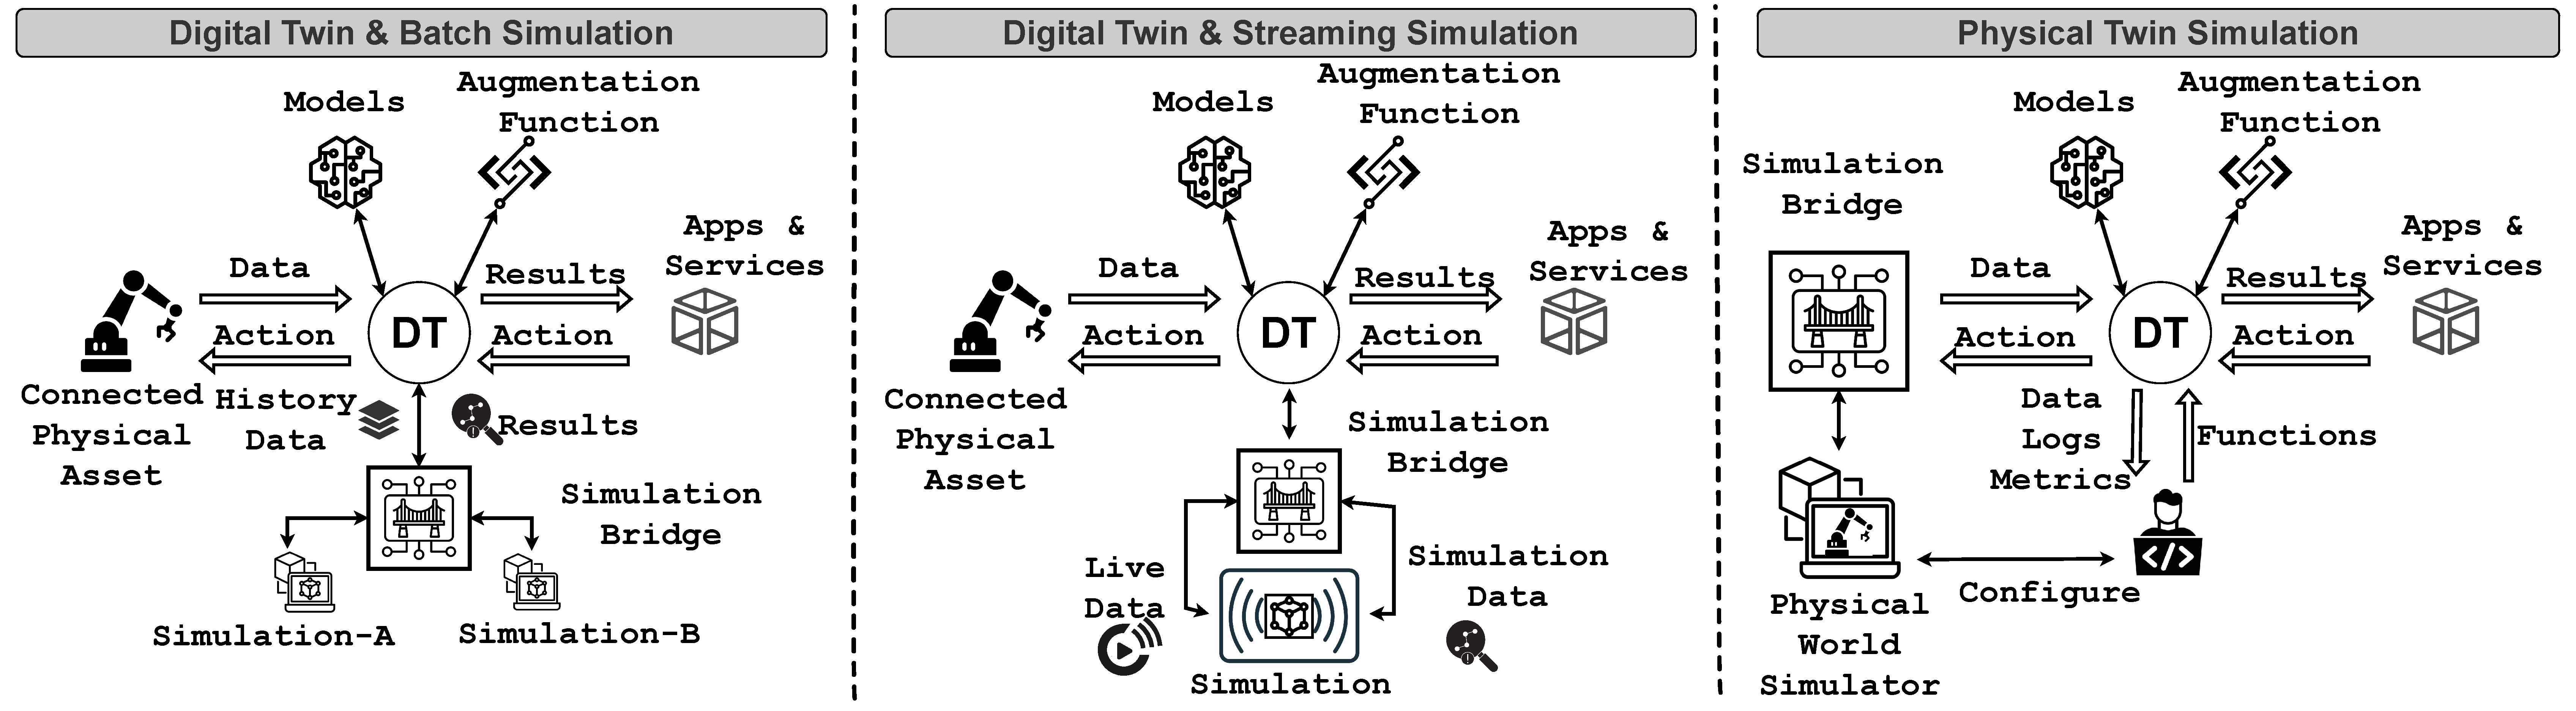
\includegraphics[width=\textwidth]{img/simulation_bridge_patterns.pdf}
    \caption{Overview of the Simulation Bridge enabling diverse interaction patterns between DTs and simulation environments.}
    \label{fig:dt_simulation_patterns}
    \vspace{-0.5cm}
\end{figure*}


\textit{(1) Enabling predictive and prescriptive capabilities.}  
While IoT-based DTs effectively capture the current state of physical systems through real-time data, open challenges remain in enhancing their ability to forecast future behavior and reason under uncertainty \cite{10015420}.
Simulation enhances DTs with predictive capabilities, supporting analysis under varying conditions such as equipment degradation, workload fluctuations, or environmental stressors~\cite{KLEIN2026103063}.
This shifts DTs from descriptive digital replicas to prescriptive and prognostic systems capable of anticipating outcomes and triggering proactive interventions.

\textit{(2) Coordinating heterogeneous simulations for complex systems.}  
Modeling complex systems often requires the orchestration of multiple, domain-specific simulations, each representing a different aspect of the physical system---e.g., mechanical dynamics, thermal effects, electrical behavior, or environmental interactions~\cite{10.1115/1.4049861,Fitzgerald2019}.
These simulations may operate at different time scales, resolutions, or levels of abstraction and must be integrated to ensure coherence and consistency. This is outside the scope of this paper.
%For example, a smart manufacturing DT might combine the kinematics of robotic arms with thermal simulations of material processing. 


\textit{(3) Supporting DT development in the absence of the Physical Twin (PT).}  
In many scenarios -- such as early-stage design, safety-critical applications, or high-cost manufacturing -- the physical system may not yet exist, be inaccessible, or pose operational risks.
In these cases, simulations -- e.g., of the IoT system~\cite{7568309} -- can act as surrogate PTs, generating mock behaviors and interaction patterns that allow the DT to be developed, tested, and validated in isolation~\cite{AITALLA20191331, 11087838}.

\textit{(4) Sharing simulation data across multiple DTs.}  
A single simulation model can serve multiple DTs, each potentially operating at different levels of abstraction and granularity.
For instance, a simulation of a production line may provide relevant data to DTs representing individual subsystems, such as robots or sensors, each requiring different views, resolutions, and update semantics. 

Despite these promising capabilities, the state of the art reflects only a partial integration of DTs and simulations~\cite{WOOLEY2023940}.
This paper presents the \emph{DT Simulation Bridge (DT-SB)}, a software framework designed to integrate DTs with multiple, heterogeneous simulation environments. The DT-SB enables bidirectional data exchange and supports diverse interaction patterns, allowing simulations to dynamically update the DT's internal state, while DTs can influence and tune simulation parameters in real time.

Unlike traditional co-simulation frameworks~\cite{Gomes&18}, the DT-SB connects a DT with multiple, independent simulations and acts solely as an intermediary. The coordination and aggregation of simulation results are delegated entirely to the DT, preserving architectural decoupling and maximizing flexibility.

We describe the modular architecture and core software components of the DT-SB, emphasizing its interoperability with diverse simulation models and protocols.

An experimental evaluation demonstrates the bridge’s effectiveness in accelerating iterative design cycles, facilitating virtual commissioning, and enabling live behavioral analysis under realistic operational conditions.


% The rest of the paper is organized as follows: Section~\ref{sec:relatedwork} reviews related work on DT–simulation integration, co-simulation, and distributed simulation frameworks. Section~\ref{sec:dt_sim_bridge} introduces the main interaction patterns supported by the DT-SB, highlighting their relevance across the DT lifecycle. Section~\ref{sec:sim_bridge_arch} presents the internal architecture of the DT-SB, detailing its modular components and communication mechanisms. Section~\ref{sec:sim-agents} describes the design and implementation of simulation agents, with particular focus on MATLAB and AnyLogic. Section~\ref{sec:experimental_evaluation} reports on the experimental evaluation of the DT-SB and its agents, analyzing latency and communication overhead. Finally, Section~\ref{sec:conclusion} summarizes the contributions and outlines directions for future work.

\section{Related Work}
\label{sec:relatedwork}

Simulation is a key technology in DTs, envisioned as a tool that can be adopted across all phases of the PT lifecycle~\cite{Boschert2016}.
%
Despite the strong overlap between simulation and DTs making it difficult to draw a line between the technologies~\cite{WOOLEY2023940}, it is becoming more and more clear that, especially in the IoT domain, DTs extend the capability of ``static'' simulations by incorporating real-time data~\cite{PHANDEN2021174}.

Most DT simulations integrate simulators and IoT data processing with custom architectures and ad-hoc methods, lacking principled integration. The DT Simulation Bridge integrates and orchestrates multiple simulations with different models in a coherent framework.
%
At a surface level, it is then similar to distributed simulation~\cite{2000daglib} and co-simulation~\cite{Gomes&18}. 
%
There are, though, fundamental differences in the approach.
%
Distributed simulation usually concerns the execution of a single complex simulation on distributed nodes.
%
Differently, co-simulation explores the possibility of composing different simulation models of individual parts to simulate a complex system and coordinate the progress of time between the different independent simulation units.
%
The purpose of the DT Simulation Bridge is, instead, to connect one DT with multiple simulations.
%, independent from one another.
%
The coordination and combination of such simulation results are expected to be managed by the DT and not by the bridge itself, which only acts as an intermediary.
%
Nevertheless, despite these differences in purposes, there are some significant aspects from these two related areas which influence the design of the bridge. 

Integrating simulations requires standardising the interaction across components.
%
For distributed simulation, the High-Level Architecture (HLA) defines a set of constraints to design interoperable federations of simulations which can be executed on a distributed runtime infrastructure~\cite{568652}.
%
Despite in our case simulations do not need to exchange data between each other, the need for a standardized interface is essential to allow the DT to seamlessly interact with multiple different simulations.
%
Similarly, in the co-simulation domain, the Functional Mockup Interface (FMI) is an industrial de facto standard \cite{FMIStandard2.0} to bridge different simulation models.
%
There, models of different nature may declare connection points to create input/output chains which combine the output of individual solvers.
%
We follow this principle in the design of the DT-SB to support simulation models which can be updated over time with the data that is captured by the DT itself. 
\section{Simulation Bridge Interaction Patterns}
\label{sec:dt_sim_bridge}

The integration of DTs with simulation environments enables a range of interaction patterns designed to support different phases of the system lifecycle and corresponding operational requirements. These interaction patterns are characterized by bidirectional data exchange and control flow, allowing DTs to incorporate predictive capabilities while simulations remain continuously informed by real-time contextual updates.
Building on the DT-SB architecture, we identify three primary interaction paradigms: \emph{Digital Twin \& Batch Simulation}, \emph{Digital Twin \& Streaming Simulation}, and \emph{Physical Twin Simulation}, as illustrated in Figure~\ref{fig:dt_simulation_patterns}. Each paradigm serves distinct objectives, encompassing design validation, what-if scenario analysis, live system adaptation, and virtual commissioning.
Together, they provide a flexible framework for coupling DTs with simulation processes across the development and operational spectrum.


\paragraph{Batch Simulation}
\label{ssec:dt-batch-simulation}

Leverages one-shot simulation runs to analyze scenarios or validate design decisions related to the DT and its physical counterpart. Acting as an intermediary, the DT-SB receives inputs from the DT, such as the current system state, historical data, or scenario configuration parameters and subsequently triggers one or more simulation runs accordingly. These batch simulations execute to completion producing results that the DT-SB forwards back to the DT.
%For instance, a DT of a manufacturing robot may employ batch simulations to evaluate the effects of various arm configurations on cycle time and energy consumption. Similarly, a DT representing a power grid might conduct ``what-if'' analyses to assess the impact of sudden demand surges or component failures on grid stability.
The resulting simulation outcomes enable the DT to refine its models, develop predictive maintenance schedules, and recommend adjustments. This pattern is particularly well suited for use cases requiring comprehensive, offline evaluations, such as design validation and strategic scenario planning.


\paragraph{Streaming Simulation}
\label{ssec:dt-streaming-simulation}

Facilitates dynamic interactions between the DT and the simulation environment through continuous data exchange. In this mode, the DT streams high-frequency operational data to the DT-SB, which relays it to a connected simulation that dynamically adapts its model based on the incoming input. The simulation continuously produces output data that is streamed back to the DT through the DT-SB.
This interaction enables live behavioral analysis and adaptive control.
%For example, a DT of a wind turbine can stream sensor data to a simulation predicting fatigue life under current wind loads; simulation results subsequently inform real-time pitch adjustments to optimize turbine health. Similarly, in smart buildings, a DT can supply HVAC sensor data to an energy optimization simulation, enabling real-time control commands to minimize energy consumption based on predicted occupancy and weather conditions.
Furthermore, deviations between live DT data and simulation outputs can serve as early indicators of anomalies or faults, thereby enabling proactive intervention.
This pattern is particularly well suited for applications demanding immediate feedback and continuous system optimization.


\paragraph{Physical Twin Simulation}
\label{ssec:physical-twin-simulation}

Involves the use of a simulation environment that functions as a digital replica of the PT.
%a physical entity or environment often referred to as a \emph{Physical Twin} (PT).
This interaction mode is particularly valuable for virtual commissioning, operator training, and control logic testing, where system behaviors can be evaluated in a safe, simulated setting prior to deployment in the real world.
In this pattern, the DT is unaware of the fact that it is communicating with a simulator and exchange data and control commands that are actuated in the simulated environment.
DT developers can configure simulation parameters through the DT-SB in order to test the behavior of the DT under varying conditions.
% In this pattern, the DT interacts with the simulator through the DT-SB, configuring simulation parameters, initiating test scenarios, and issuing control commands. The simulator, in turn, provides logs, metrics, and state feedback to the DT, effectively representing the outcomes of these interactions.
%
% For instance, prior to deploying a new production line, its DT may control a simulated model of the line to evaluate control algorithms, identify bottlenecks, and optimize throughput—without risking downtime or production losses.
% Similarly, operators can train in DT-driven virtual environments, rehearsing complex procedures or emergency protocols without exposing actual equipment to risk.
This pattern enables thorough testing and validation within a controlled virtual environment, significantly reducing the costs and risks associated with physical prototyping and on-site experimentation.

\begin{comment}
\begin{figure}[h]
    \centering
    %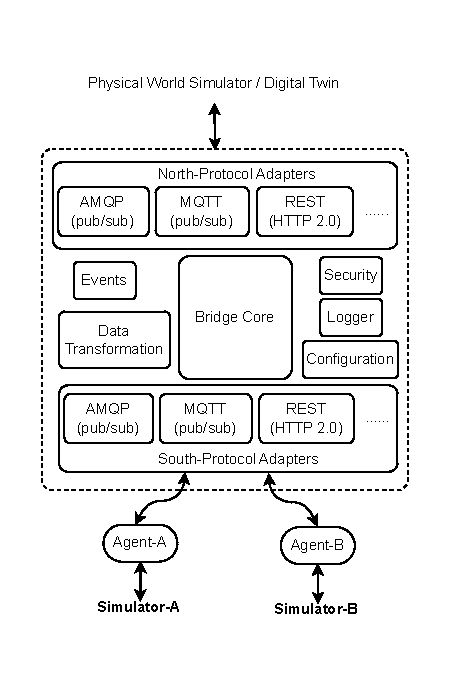
\includegraphics[width=\linewidth]{img/simulation_bridge.pdf}
    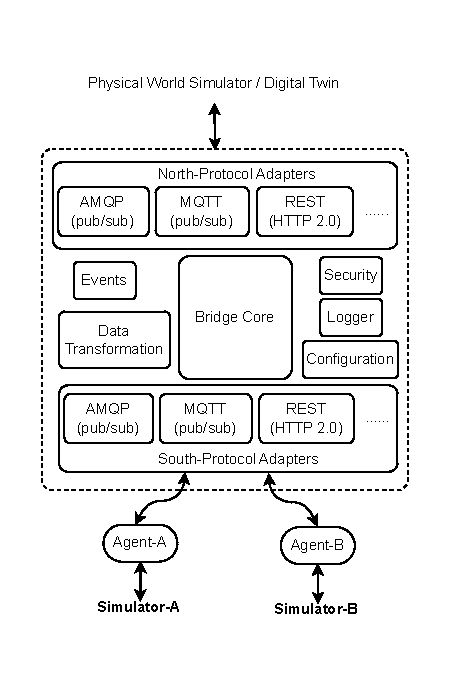
\includegraphics[width=0.7\linewidth, trim={0.1in 0.5in 0.1in 0.5in}, clip]{img/simulation_bridge.pdf}
    \caption{Architecture of the simulation bridge.}
    \label{fig:simulation_bridge_architecture}
\end{figure}   
\end{comment}

\begin{figure*}[h]
    \centering
    \subfloat[Simulation bridge architecture.]{
        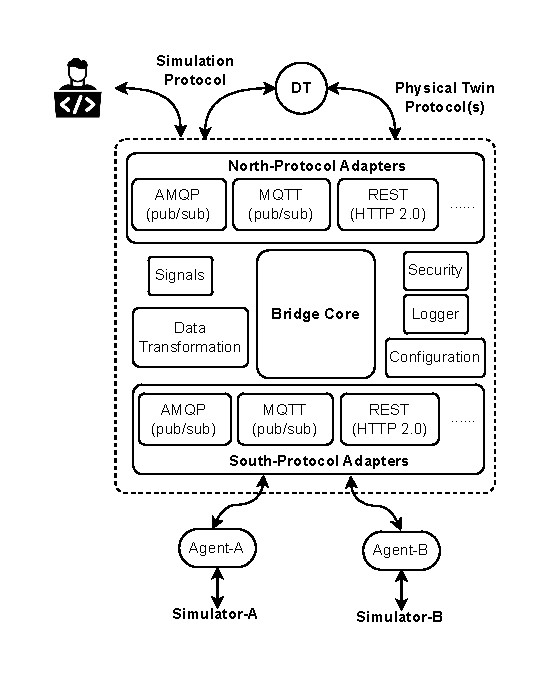
\includegraphics[width=0.35\linewidth]{img/simulation_bridge_v2.pdf}
        \label{fig:simulation_bridge_components}
    }
    \hfill
    \subfloat[Communication flow in the simulation bridge.]{
        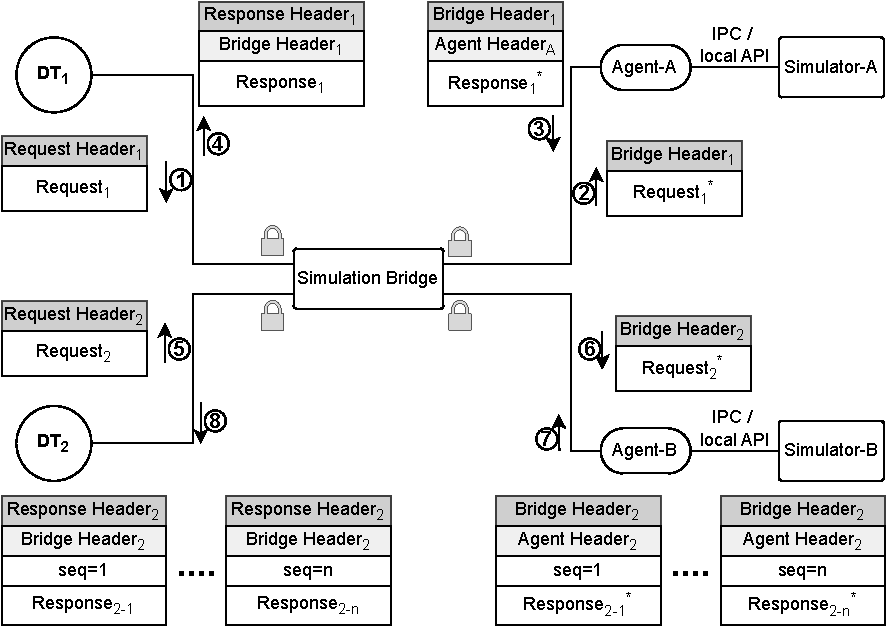
\includegraphics[width=0.56\linewidth]{img/network-setup.pdf}
        \label{fig:simulation_bridge_protocol}
    }
    \caption{Architecture of the Simulation Bridge with its main components and the associated interaction flows.}
    % \Description{Architecture of the Simulation Bridge: (a) modular components supporting DT interaction and developer-driven PT simulation, and (b) communication flow between DTs, the bridge, and simulators for simulation control and integration.}
    \label{fig:simulation_bridge_architecture}
    \vspace{-0.5cm}
\end{figure*}


\section{Simulation Bridge Architecture}
\label{sec:sim_bridge_arch}

The DT-SB coordinates heterogeneous and distributed simulations, providing a unified interface for DTs to access diverse simulation resources regardless of modeling and technological differences.
The bridge serves as a middleware which routes simulation execution requests, aggregates results, and returns them to clients. This enables seamless integration, reusability, and interoperability across simulation platforms.
% The DT-SB is designed to manage and execute heterogeneous and distributed simulations, serving as a middleware layer that facilitates interaction between DTs and a federation of simulators.
% Its primary objective is to offer a unified interface through which clients, namely DTs, can interact with a diverse set of simulation resources. 
% These simulators vary widely in their engineering paradigms, modeling approaches, and underlying implementation technologies.
% To address this diversity, the DT-SB operates as an intelligent coordination layer, responsible for routing client requests to the appropriate simulators, aggregating the resulting data, and delivering it back to the requesting clients.
% This abstraction enables seamless integration and orchestration of simulation services across heterogeneous platforms, fostering reusability, scalability, and interoperability within DT-driven ecosystems.

Figure~\ref{fig:simulation_bridge_components} illustrates the modular architecture of the DT-SB. 
At the heart of this architecture is the DT-SB, each simulator is integrated through a dedicated simulation agent (SA) module.
SAs implement a standardized uniform API layer based on a simple application protocol. 
These agents are deployed within their respective simulation environments and are responsible for interpreting incoming messages, controlling the execution of simulation tasks, and aggregating the results for transmission back to the DT-SB.
% This agent-based design ensures system-wide interoperability and enables seamless coordination across a diverse set of simulation environments.
%
Each module of the DT-SB is designed to fulfill a specific function within the operational workflow:
%. A concise description of the principal components is provided below.

\noindent\textbf{Bridge Core:}  
Serves as the central control unit of the DT-SB. It coordinates interactions among internal modules, monitors communication flows, and orchestrates message routing between external clients (e.g., DTs, PTs, simulators) and the distributed simulation environment.

\noindent\textbf{Protocol Adapters (PAs):}  
facilitate protocol translation and connection management between the DT-SB and external entities. They operate on both the north-bound interface (connecting to DTs and PTs) and the south-bound interface (connecting to SAs). PAs are implemented using a plugin architecture, allowing the system to be extended in a modular fashion.

\noindent\textbf{Event Manager:}  
DT-SB adopts an event-driven architecture, wherein all relevant actions within a PA (e.g., message transmission, reception, connection management) are internally represented as events. When a request or response is received by a PA, it is transformed into an internal event and processed by the Bridge Core.

\noindent\textbf{Data Transformation Manager:} 
is responsible for converting data formats for both incoming and outgoing communication. Transformation parameters are dynamically configurable to optimize message structures for transmission efficiency. The module supports configurable message granularity, enabling the system to manage both atomic events and composite result packets based on application requirements.

\noindent\textbf{Configuration Manager:}  
handles the validation and loading of system parameters, including supported protocols, access credentials, and routing rules. A centralized configuration approach facilitates maintainability and control. The configuration also specifies a whitelist of authorized DTs and SAs.
%, where DTs are identified via client identifiers and SAs by the \emph{simulation types} they support.
%Simulation types abstract the behavior of the DT by combining models with associated simulation methods. While DTs may specify models for simulation, local configurations may influence execution behavior even with a given model-simulator pairing.

\noindent\textbf{Logger:}  
records internal operations, exceptions, and diagnostic messages. It also provides performance metrics and operational insights essential for monitoring and debugging the DT-SB.

\noindent\textbf{Security Manager:}  
oversees the generation and loading of TLS certificates, ensuring secure communication channels. It is also responsible for detecting and mitigating malicious activity, such as message flooding, that could lead to denial-of-service conditions targeting simulators.

\subsection{Simulator Protocol}
\label{subsec:sim-protocol}

As DTs, DT-SB, and SAs operate in a distributed system, a dedicated \emph{Simulation Protocol} (SP) serves as the unifying layer for managing simulation requests and responses. The protocol defines standard headers for request routing and result interpretation. PAs integrated into DT-SB provide their own delivery semantics; however, best-effort delivery is universally supported, making it a practical foundation for interactions with SAs. Simulators can advertise the \emph{Simulation Type (ST)} they support (an abstraction that defines expected behaviors and model-method combinations). DTs may then select one of the available STs, while the DT-SB is responsible for routing and translating the corresponding simulation requests to the appropriate SAs that provide the selected ST.

The DT-SB performs two key operations to mediate this interaction:
(i) \emph{data transformation} of simulation requests and responses to ensure syntactic and semantic consistency, and
(ii) \emph{protocol header replacement} to enforce proper message routing between DTs and the selected SAs.
Figure~\ref{fig:simulation_bridge_protocol} depicts the message exchange flow for both batch and streaming simulation modes.
Secure variants of PAs are also illustrated. 
Numbered arrows indicate the sequence of message exchanges.


\paragraph{Batch Request}
In this scenario, $DT_1$ issues a simulation request targeting a Simulation Type supported by \emph{Simulator-A} (message $m_1$, denoted as \textcircled{1} in Figure~\ref{fig:simulation_bridge_protocol}). The request includes the model name, associated model parameters, simulator input values, and the specification of required outputs.
Upon receiving the request, the DT-SB replaces the original request header with a bridge-specific header. This header replacement ensures the necessary abstraction and transparency between DTs and SAs, decoupling clients from simulator-specific implementations. The DT-SB also performs a data transformation step to normalize the request format before forwarding it to \emph{Agent-A} (message $m_2$).
Agent-A then transmits the transformed request to \emph{Simulator-A}, which executes the simulation. The resulting outputs are sent back to the DT-SB via Agent-A (message $m_3$). Agent-A attaches a custom response header containing metadata relevant to the simulation run.
Upon receiving the response, the DT-SB applies a reverse data transformation tailored to the expectations of $DT_1$, replaces the agent-specific header with a standardized response header derived from the original request metadata, and delivers the final message to $DT_1$ (message $m_4$).
All headers in the message exchange carry metadata useful for distributed tracing, debugging, and performance analysis, thereby supporting observability and diagnostics across the system.


\paragraph{Streaming Request}
In this scenario, $DT_2$ initiates a simulation request targeting \emph{Simulator-B} (message $m_5$, denoted as \textcircled{5} in Figure~\ref{fig:simulation_bridge_protocol}). As with batch requests, the DT-SB intercepts the request, applies the necessary data transformation, and replaces the header with a bridge-specific version before forwarding the request to \emph{Agent-B} (message $m_6$). Agent-B then relays the request to \emph{Simulator-B}, which begins executing the streaming simulation.
Unlike batch simulations, streaming simulations generate a sequence of response messages over time. To ensure that responses are interpreted in the correct order, Agent-B attaches a sequence number to each outgoing message. This sequence number enables both DT-SB and $DT_2$ to preserve the temporal order of the response stream.
Agent-B forwards the ordered sequence of responses to the DT-SB (denoted as multiple instances of message $m_7$), which in turn applies reverse data transformation and forwards the processed responses to $DT_2$ (messages $m_8$).
In Figure~\ref{fig:simulation_bridge_protocol}, these streaming responses have $seq$ number field which is used by $DT_2$ to arrange the streaming responses in the correct order.

\paragraph{PT Simulation}

For the simulation of PTs, the DT-SB is used by two distinct entities. On one side, the developer interacts with the bridge through the simulation protocol and the north-protocol adapters to configure and launch simulations, define the mapping of simulated entities, and specify how these entities are exposed to the digital world via specific protocols, for example by mapping a simulation entity to MQTT. On the other side, the DT receives data from the simulated PTs through the configured protocols as if it were coming from the actual physical objects that will feed the DT in real deployments. Communication between the DT and the DT-SB is bidirectional: the DT not only receives telemetry data from the simulated PTs but can also send actions. These actions are translated by the bridge into commands for the simulation, modifying the behavior of the simulated PTs via interactions managed through the protocols and simulation agents enabled by the south-protocol adapters.


%\hl{hard to match the stuff below with figure}

\begin{comment}
In Figure~\ref{fig:simulation_bridge_protocol}, these responses are labeled as $Response_{2\text{-}k}$, where the first subscript ($2$) denotes the originating DT (i.e., $DT_2$), and the second subscript ($k$) denotes the position in the response sequence. Both DT-SB and $DT_2$ rely on the sequence number embedded in each response to ensure correct processing and ordered delivery of simulation outputs.
\end{comment}


\subsection{Routing Messages}

%Simulators often expose non-standard interfaces, which vary significantly in terms of programming abstractions and platform dependencies. Some simulators offer APIs in high-level programming languages, while others provide operating system-specific bindings. For instance, \emph{Matlab} exposes a Python API, whereas \emph{Simul8} provides a COM-based interface that is limited to the Windows operating system. Additionally, several simulators support traditional inter-process communication (IPC) mechanisms such as files, named pipes, network sockets, and shared memory. Among these, shared memory enables the most tightly coupled integration between SAs and the simulator, offering low-latency, high-throughput communication. In contrast, network socket-based interfaces allow greater deployment flexibility by enabling the SA and its associated simulator to reside on different nodes within a distributed system.

A critical responsibility of the DT-SB is to map incoming simulation responses to their corresponding requests. This mapping is maintained using a dynamic routing table, with representative entries illustrated in Table~\ref{tab:index-table}. 

\begin{table}[h]
    \centering
    \caption{DT-SB's routing table.}
    \label{tab:index-table}
    \renewcommand{\arraystretch}{1.5}  % Adjust this factor to achieve 12pt spacing
    \begin{tabular}{p{0.5in}llp{0.5in}lp{0.5in}}
    \hline
    \textbf{$PA_N$} & \textbf{$PA_S$} & \textbf{DT} & \textbf{Sim. Type} & \textbf{Request-id} & \textbf{Timeout}\\
    \hline
    MQTT & AMQP & $DT_1$ & Octave & $hash\#1$ & 60s\\
    AMQP & MQTT & $DT_1$ & Matlab & $hash\#2$ & 60s\\
    REST & AMQP & $DT_2$ & Simul8 & $hash\#3$ & 120s\\
    \hline
    \end{tabular}
\end{table}

% \begin{table}[h]
%     \centering
%     \caption{Routing table used by DT-SB for internal message routing.}
%     \label{tab:index-table}
%     \renewcommand{\arraystretch}{1.5}  % Adjust this factor to achieve 12pt spacing
%     \begin{tabular}{p{0.5in}llp{0.5in}lp{0.5in}}
%     \hline
%     \textbf{$PA_N$} & \textbf{$PA_S$} & \textbf{DT} & \textbf{Simulator Type} & \textbf{Request-id} & \textbf{Timeout (seconds)}\\
%     \hline
%     MQTT & AMQP & $DT_1$ & Octave & $hash\#1$ & 60\\
%     AMQP & MQTT & $DT_1$ & Matlab & $hash\#2$ & 60\\
%     REST (HTTP/2.0) & AMQP & $DT_2$ & Simul8 & $hash\#3$ & 120\\
%     \hline
%     \end{tabular}
% \end{table}

The column $PA_N$ denotes the PA selected by the DT, while $PA_S$ represents the PA associated with the Simulator Agent. In scenarios where the DT-SB supports only a single protocol on either the north-bound ($PA_N$) or south-bound ($PA_S$) interface, the corresponding column can be omitted to simplify the routing logic.
The \emph{Simulator Type} column identifies the class of simulations handled by a given SA. Each simulation request is uniquely identified by a \texttt{RequestID}, which may be generated using hash-based algorithms to ensure uniqueness and unpredictability. A timeout field is also included to define the expiration threshold for requests; expired entries are purged to maintain routing table efficiency. When a simulation response arrives, the tuple $\langle PA_S, ST, \texttt{RequestID} \rangle$ is extracted and matched against existing routing table entries. The identified row provides the target DT and the associated $PA_N$, allowing the DT-SB to correctly route the response back to the originating DT. This mechanism ensures correct correlation of simulation data even in asynchronous or distributed execution contexts.




\begin{comment}
\begin{figure}[h]
    \centering
    
\includegraphics[height=4cm]{img/event_based_sm.pdf}
    \caption{Event-Based Architecture\textcolor{blue}{replace with a table}}
    \label{fig:event_based_sm}
\end{figure}

The \textit{sim-bridge} is a sophisticated software platform involving advanced engineering challenges, designed to execute heterogeneous distributed simulations. 
Its primary goal is to enable an external client to interact in a simple and transparent way with a network of distributed simulators, which may differ significantly in terms of nature, technology, and location.

The role of the sim-bridge project is therefore to act as an intelligent intermediary between the client and the various simulators, handling the routing of incoming requests to the appropriate simulator, collecting the results, and delivering them back to the client in a secure and efficient manner. In this context, \textit{sim-bridge} not only ensures uniform access to distributed simulation resources, but also abstracts the underlying complexities arising from their heterogeneity.

\begin{figure}[h]
    \centering
    
\includegraphics[height=4cm]{img/simulation_bridge_overview.pdf}
    \caption{\textit{sim-bridge} Overview}
    \label{fig:simulation_bridge_overview}
\end{figure}    

To enable this functionality, a central component, the \textit{sim-bridge}, has been designed to handle the routing of requests across multiple communication protocols and to manage the distributed nature of the simulators. In order to be integrated into the system, each simulator requires a dedicated agent that acts as an internal interpreter between the simulator's proprietary APIs and the \textit{sim-bridge} (Figure~\ref{fig:agent_role}).

To address the challenges posed by the diversity of proprietary languages, complex connectors, and custom APIs, together with the absence of a universally accepted standard protocol, a dedicated agent has been developed for each simulator. 

Each simulator is thus paired with its own agent, which implements a common interface shared among all agents. This standardized interface defines the APIs and communication methods used to interact with the various simulators, ensuring both consistency and interoperability within the system.

\begin{figure}[h]
    \centering
    
\includegraphics[height=5cm]{img/agent_role.pdf}
    \caption{Agent Role}
    \label{fig:agent_role}
\end{figure}

Communication between clients and the \textit{Simulation Bridge} is flexible and location-independent. As depicted in Figure~\ref{fig:position_sm}, this communication can occur either directly at the client’s edge or within the system core, depending on each Digital Twin or Mock Physical Twin’s capability to support specific communication protocols.

\begin{figure}[h]
    \centering
    
\includegraphics[height=6cm]{img/position_sm.pdf}
    \caption{Communication between clients and \textit{sim-bridge}}
    \label{fig:position_sm}
\end{figure}    

\begin{figure}[h]
    \centering
    
\includegraphics[height=6cm]{img/project.pdf}
    \caption{Structure of the Simulation Bridge}
    \label{fig:structure}
\end{figure}

Figure~\ref{fig:structure} illustrates the modular architecture of the \textit{sim-bridge} and its main software components. Each module is designed to perform a specific function within the overall operational workflow.

\textbf{Protocol Adapter}

The \textit{Protocol Adapter} module is responsible for translating and managing connections between the \textit{sim-bridge} and various communication protocols. In the initial version, the \textit{sim-bridge} supports RabbitMQ, MQTT, and HTTP. This component is designed with a plugin architecture, allowing easy extension to support new protocols, thus ensuring flexibility and adaptability to future requirements.

\textbf{Data Transformation Manager}

The \textit{Data Transformation Manager} handles the transformation of incoming and outgoing data, adapting it to the formats required by simulators or production systems. This module allows configurable management of message granularity, supporting both single events and complete result packets, depending on the needs of the application context. The configurability of the transformation level enables dynamic selection of the data format and structure to be transmitted.

\textbf{Config Manager}

The \textit{sim-bridge} is fully configurable via YAML files. The \textit{Config Manager} is responsible for reading, validating, and loading this configuration file, which defines the entities involved, the protocols to be used, and the rules for message routing. This approach promotes centralized and transparent configuration management, facilitating system maintenance and scalability.

\textbf{Logger}

The system integrates a customized logger that records all internal operations and handles potential errors. The logger configuration is also managed through the YAML file, allowing adjustment of the log detail level according to different operational needs (e.g., INFO, DEBUG, WARNING, ERROR, CRITICAL).

\textbf{Certs Manager}

The \textit{Certs Manager} module is responsible for generating, validating, and managing TLS security certificates, such as certfiles and keyfiles. If these certificates are missing or invalid, the manager automatically generates and stores them in the predefined folder, thus ensuring secure communications.

\textbf{\textit{sim-bridge} Core}

The \textit{Core} represents the logical heart of the system. It coordinates the internal components, monitors real-time communications, and manages message routing between external clients and distributed simulators.

\textbf{Signal Manager}

The \textit{sim-bridge} is based on an event-driven architecture, where each protocol has both an input and an output channel, each linked to internal events. When a message arrives on a protocol, it is converted into an event and handled by the core. Similarly, results follow the same process. The \textit{Signal Manager} reads the event configuration from the file \texttt{adapters\_signal.json} and automatically associates callback functions to the corresponding events, ensuring efficient event management.
Figure~\ref{fig:event_based_sm} illustrates how each protocol adapter is connected to specific events and how the core component manages these events.

\begin{figure}[h]
    \centering
    
\includegraphics[height=4cm]{img/event_based_sm.pdf}
    \caption{Event-Based Architecture}
    \label{fig:event_based_sm}
\end{figure}


\textbf{\textit{sim-bridge} Infrastructure}

The \textit{sim-bridge} uses an internal communication infrastructure based on RabbitMQ, which is necessary for secure and structured communication with the simulator agents. The connection between the \textit{sim-bridge} and the agents is stable and exclusively maintained via RabbitMQ.

\textbf{Simulator’s Agent}

The inherent challenges associated with various proprietary languages of simulators and the absence of standardized communication protocols are mitigated through an systematic agent-based approach. Each simulator is coupled with a specialized agent that conforms to a standardized interface specification. This architectural decision establishes a uniform API layer and communication methodology for simulator interactions, thereby ensuring system-wide interoperability and maintaining consistency across the distributed simulation environment.

The integration of individual simulators into this framework is accomplished through dedicated agent modules that function as interface adapters between proprietary simulator APIs and the centralized sim-bridge architecture, as depicted in Fig. 1.

The \textit{Simulator’s Agent} is a software component developed specifically for each integrated simulator. Its purpose is to act as an intermediary between the \textit{sim-bridge} and the simulator’s proprietary APIs. Each agent implements a common, standardized interface shared by all agents, allowing the \textit{sim-bridge} to interact uniformly with heterogeneous simulators. The agent must be integrated within the simulation software itself and manages message interpretation, simulation activation, and result collection to be forwarded to the \textit{sim-bridge}.

\end{comment}




\section{Simulation Agents}
\label{sec:sim-agents}

This section presents the simulation agents integrated into the DT-SB architecture: the MATLAB and AnyLogic Agents enabling computational and simulation model execution with modularity and seamless communication.

\subsection{Matlab Agent}

The MATLAB Agent ($SA_{\text{MATLAB}}$) serves as a decoupled simulation component integrating MATLAB’s computational capabilities within the DT-SB architecture. It communicates with the DT-SB through the AMQP protocol, enabling reliable and platform-independent message exchange. Four integration strategies were explored, each balancing latency, flexibility, and architectural coupling differently. 

In the \textit{file-based approach}, simulation inputs are provided as files, and results are written back to disk for the agent to read and forward to the DT-SB. This method ensures strong decoupling but introduces considerable input/output overhead, making it unsuitable for real-time or streaming simulations. The \textit{TCP/IP communication approach} enables real-time data exchange via socket-based interprocess communication, where results are transmitted as JSON messages. This solution supports continuous streaming and distributed deployment with moderate latency. A third strategy relies on shared memory \textit{interprocess communication}, where requests and responses are exchanged directly through memory segments. While this configuration achieves minimal latency and high throughput, it requires explicit synchronization and strict control over memory layout, reducing flexibility. Finally, the MATLAB Engine API allows direct invocation of MATLAB functions from Python, simplifying model execution but imposing tighter structural constraints and lowering modularity.

Experimental evaluation showed that shared memory communication provides the lowest latency but lacks adaptability. Therefore, the MATLAB Engine API was selected for \emph{batch} simulations, whereas the TCP/IP approach was adopted for \emph{streaming} mode, offering a balanced trade-off between performance, modularity, and ease of integration.

%%%%%%%%%%%%%%%%%%%%%%%%%%%%%%%%%%%%%%%%%%%%%%%%%%%%%%%%%
% The MATLAB Agent ($SA_{\text{MATLAB}}$) represents a decoupled simulation agent that integrates MATLAB's computational capabilities within the DT-SB architecture. The agent communicates with the DT-SB using the AMQP protocol, ensuring reliable and platform-agnostic messaging. Four distinct integration strategies were investigated, each offering different trade-offs in terms of latency, flexibility, and architectural coupling.

% \textbf{1. File-Based Exchange.}
% In this approach, the simulator receives simulation inputs via files, executes the model, and stores the results in an output file. The $SA_{\text{MATLAB}}$ reads the output file, encapsulates its contents as the response payload, and forwards the message to the DT-SB. This method offers high architectural decoupling but incurs substantial input/output overhead, making it unsuitable for streaming simulations due to poor performance and high latency.

% \textbf{2. TCP/IP Communication.}
% This approach employs network-based IPC, enabling real-time interaction between the simulator and the $SA_{\text{MATLAB}}$. The simulator sends result data directly to the $SA_{\text{MATLAB}}$ over a TCP/IP socket, formatted as JSON. Each result corresponds to a single message in the stream, making this method highly compatible with streaming simulation modes. The use of network IPC ensures that the MA and simulator remain decoupled at the operating system process level, supporting distributed deployment.

% \textbf{3. Shared Memory IPC.}
% In this configuration, the $SA_{\text{MATLAB}}$ and MATLAB exchange data via shared memory segments. Simulation requests and responses are written and read directly from volatile memory, resulting in extremely low latency and high throughput. However, this approach requires explicit synchronization using mutexes or locks to avoid race conditions and deadlocks. Additionally, shared memory access necessitates strict control over memory layout, reducing flexibility.

% \textbf{4. MATLAB Engine API.}
% This method utilizes the MATLAB Engine API to directly invoke MATLAB functions from Python. While it simplifies invocation of MATLAB computations, it imposes structural constraints on model definitions and requires the simulator to conform to specific function-call semantics, thus reducing modularity and reusability.

% A comprehensive evaluation of these four approaches has been conducted to determine the most suitable integration strategy for \emph{batch} and \emph{streaming} simulation modes. Although shared memory IPC achieves the lowest latency, it required rigid memory management and offers limited flexibility.
% Ultimately, the Matlab Engine API approach has been selected for batch simulation. The TCP/IP approach has been selected as the preferred integration method for streaming mode simulation due to its balance of modularity, ease of integration, and suitability for distributed architectures.

%%%%%%%%%%%%%%%%%%%%%%%%%%%%%%%%%%%%%%%%%%%%%%%%%%%%%%%%%%%

%$SA_{\text{MATLAB}}$ supports both \emph{batch} and \emph{streaming} simulation modes. In batch mode, the agent invokes complete MATLAB routines using parameters provided at initialization, returning only the final output upon completion of the simulation.
%In contrast, streaming mode facilitates continuous, unidirectional data exchange during simulation execution via TCP/IP communication channels. During streaming simulations, $SA_{\text{MATLAB}}$ communicates with MATLAB over the TCP protocol, transmitting the simulation parameters and a reference to the model file. The agent does not participate in the execution of the MATLAB model itself; it solely manages data exchange and response handling. This separation of concerns preserves architectural modularity and ensures a clear boundary between model execution and communication infrastructure.


\begin{comment}

The MATLAB Agent represents a specialized implementation of decoupled simulation agent designed to seamlessly integrate MATLAB functionalities into the \textit{sim-bridge} system. As the first simulation agent developed in the context of this research, it serves a dual role: both as an operational component and as an architectural reference for designing future agents within the component-based \textit{sim-bridge} framework.

Implemented as a Python package installable via pip, the agent can operate independently or in direct coordination with the \textit{sim-bridge}, acting as an interpreter between standardized simulation requests and the MATLAB execution environment. Communication is handled through RabbitMQ, selected for its compatibility with the \textit{sim-bridge} infrastructure and its ability to manage asynchronous communication in distributed systems.

The architecture of the MATLAB Agent comprises four core modules:
\begin{itemize}
    \item \textbf{Configuration Manager:} centralizes parameter management through external YAML files, facilitating configuration and reusability.
    \item \textbf{RabbitMQ Manager:} handles asynchronous communication with the external environment, particularly the \textit{sim-bridge}.
    \item \textbf{Simulation Handlers:} implement two operational modes—batch and streaming—to address different computational needs.
    \item \textbf{Logging \& Error Handling:} ensures operational reliability through detailed logging and structured error management.
\end{itemize}
This modular design supports both one-off parametric studies and continuous real-time simulations, as typically required in digital twin applications.

\paragraph{Operational Modes}
The agent supports two primary execution modes:
\begin{itemize}
    \item \textbf{Batch Mode:} Executes complete MATLAB routines using parameters provided at initialization. Ideal for validation scenarios, where simulation outputs support system-level decisions. Data is provided once at simulation start, and the output is returned in structured form at the end. Functions must comply with a predefined signature, such as:
\begin{verbatim}
function [output1, output2] = simulation(input1, input2, input3)
% Simulation logic
end
\end{verbatim}

    \item \textbf{Streaming Mode:} Enables continuous data exchange during execution, supporting real-time feedback cycles. It is well-suited for MockPT environments, where a simulated PT must be emulated. Communication occurs via TCP/IP channels managed by an interface called \texttt{SimulationWrapper}, which enables persistent data exchange at each simulation step.
\begin{verbatim}
function Simulation()
wrapper = SimulationWrapper(); % Initialization
inputs = wrapper.get_inputs(); % Retrieve initial inputs

while simulation_running
    data = compute_step(inputs); % Compute simulation step
    wrapper.send_output(data);   % Send real-time output
end

delete(wrapper); % Resource cleanup
end
\end{verbatim}
Using \texttt{SimulationWrapper} is not mandatory but strongly recommended to ensure compatibility with the agent's communication interface. It manages TCP communication with the agent automatically.
\end{itemize}    

\paragraph{Communication Strategies Analysis}
A critical performance aspect is the efficiency of communication between the agent and MATLAB. Four strategies were evaluated:
\begin{enumerate}
    \item \textbf{.mat file exchange:} High decoupling but significant I/O overhead, unsuitable for high-frequency applications.
    \item \textbf{MATLAB Engine API:} Direct communication with good performance but enforces structural constraints on MATLAB functions.
    \item \textbf{TCP/IP Communication:} Real-time interaction using JSON, maintaining process independence.
    \item \textbf{Shared Memory IPC:} Lowest latency but requires predefined memory layouts, reducing flexibility.
\end{enumerate}
TCP/IP was selected as the optimal trade-off, offering modularity, ease of integration, and support for distributed scenarios. The performance overhead is minimal, and adding the \texttt{SimulationWrapper} module ensures full interoperability.

\paragraph{Integration in the Digital Twin Ecosystem}
Within the broader architecture, the MATLAB Agent acts as a specialized computational node, capable of executing complex numerical simulations while interfacing seamlessly with other system components. Simulation requests are received via the \textit{sim-bridge}, processed using MATLAB, and results are returned according to the expected data flow. This integration leverages the entire MATLAB ecosystem, including Simulink and all available Toolbox components.
\end{comment}



\subsection{AnyLogic Agent}

AnyLogic\footnote{AnyLogic: \url{https://www.anylogic.com/}}, is a flexible simulation platform that combines agent-based, discrete-event, and system dynamics modeling.
This versatility makes it ideal for creating detailed digital representations of industrial CPSs.
%
We hence develop the agent to support the PT simulation pattern. 

The AnyLogic Agent has two components:
1) an interface to the DT-SB which accepts simulation requests and configures the AnyLogic scenario accordingly. Differently from the other patterns, these requests come from the DT developer who wants to test the DT behaviour on a simulated PT;
2) a general purpose \emph{entity}\footnote{We use \emph{entity} here to avoid overloading the term agent. Since AnyLogic is an agent-based simulator, all entities within the simulations are modeled as agents which can exchange messages using built-in mechanisms.} that can be embedded within the simulation to receive messages from other entities and serialize them on a network socket to output a data stream of relevant events happening within the simulation. The simulation data stream is then received from the south protocol adapters, and routed to the physical interface of the DT with the north protocol adapters (Fig. \ref{fig:simulation_bridge_components}).

The AnyLogic data stream carries information about which simulation entity generated it, which can be used by the bridge to map the corresponding update on a different protocol for the DT.
This design is needed to emulate scenarios where data about one or more PTs is sent over different communication protocols (e.g. a sensor network), making it possible to test the DT simply by changing its configuration to point to the emulated communication channels and leaving all the connection handling and message processing logic unaltered.
The connection is bi-directional, to allow the DT to send control commands and apply them onto the simulated PT.


% \hl{everything below is already explained above when we talk about the DT-SB and should be removed. here we describe specific details of the agents! take inspiration from the matlab agent part. }

% The connection with the DT-SB is managed through a \textit{Bridge Connection} component, responsible for maintaining an active link with the DT-SB. This component intercepts simulation events, identifies the entity generating the event (e.g., the robot moving a product), and propagates the data in a structured format while preserving the unique identifier of the source within the simulation.
% The same mechanism handles incoming messages from external systems, transforming them into simulation events and delivering them to the appropriate element.
% This design allows the Bridge Connection to operate in parallel with the existing simulation elements and to be activated at key points where integration with the DT-SB is required, e.g., to emulate the behavior of a PT.

% Each element is associated with dedicated message structures for telemetry (e.g., state, position, status) and actions (e.g., commands, control inputs). These messages are granularly mapped to the protocols supported by the DT-SB (via its north-protocol adapters), ensuring compatibility with diverse DT frameworks. This design supports high-fidelity PT emulation, live interaction, and flexible testing of configurations and scenarios through bidirectional communication.
\begin{comment}
\begin{figure}[ht]
    \centering
    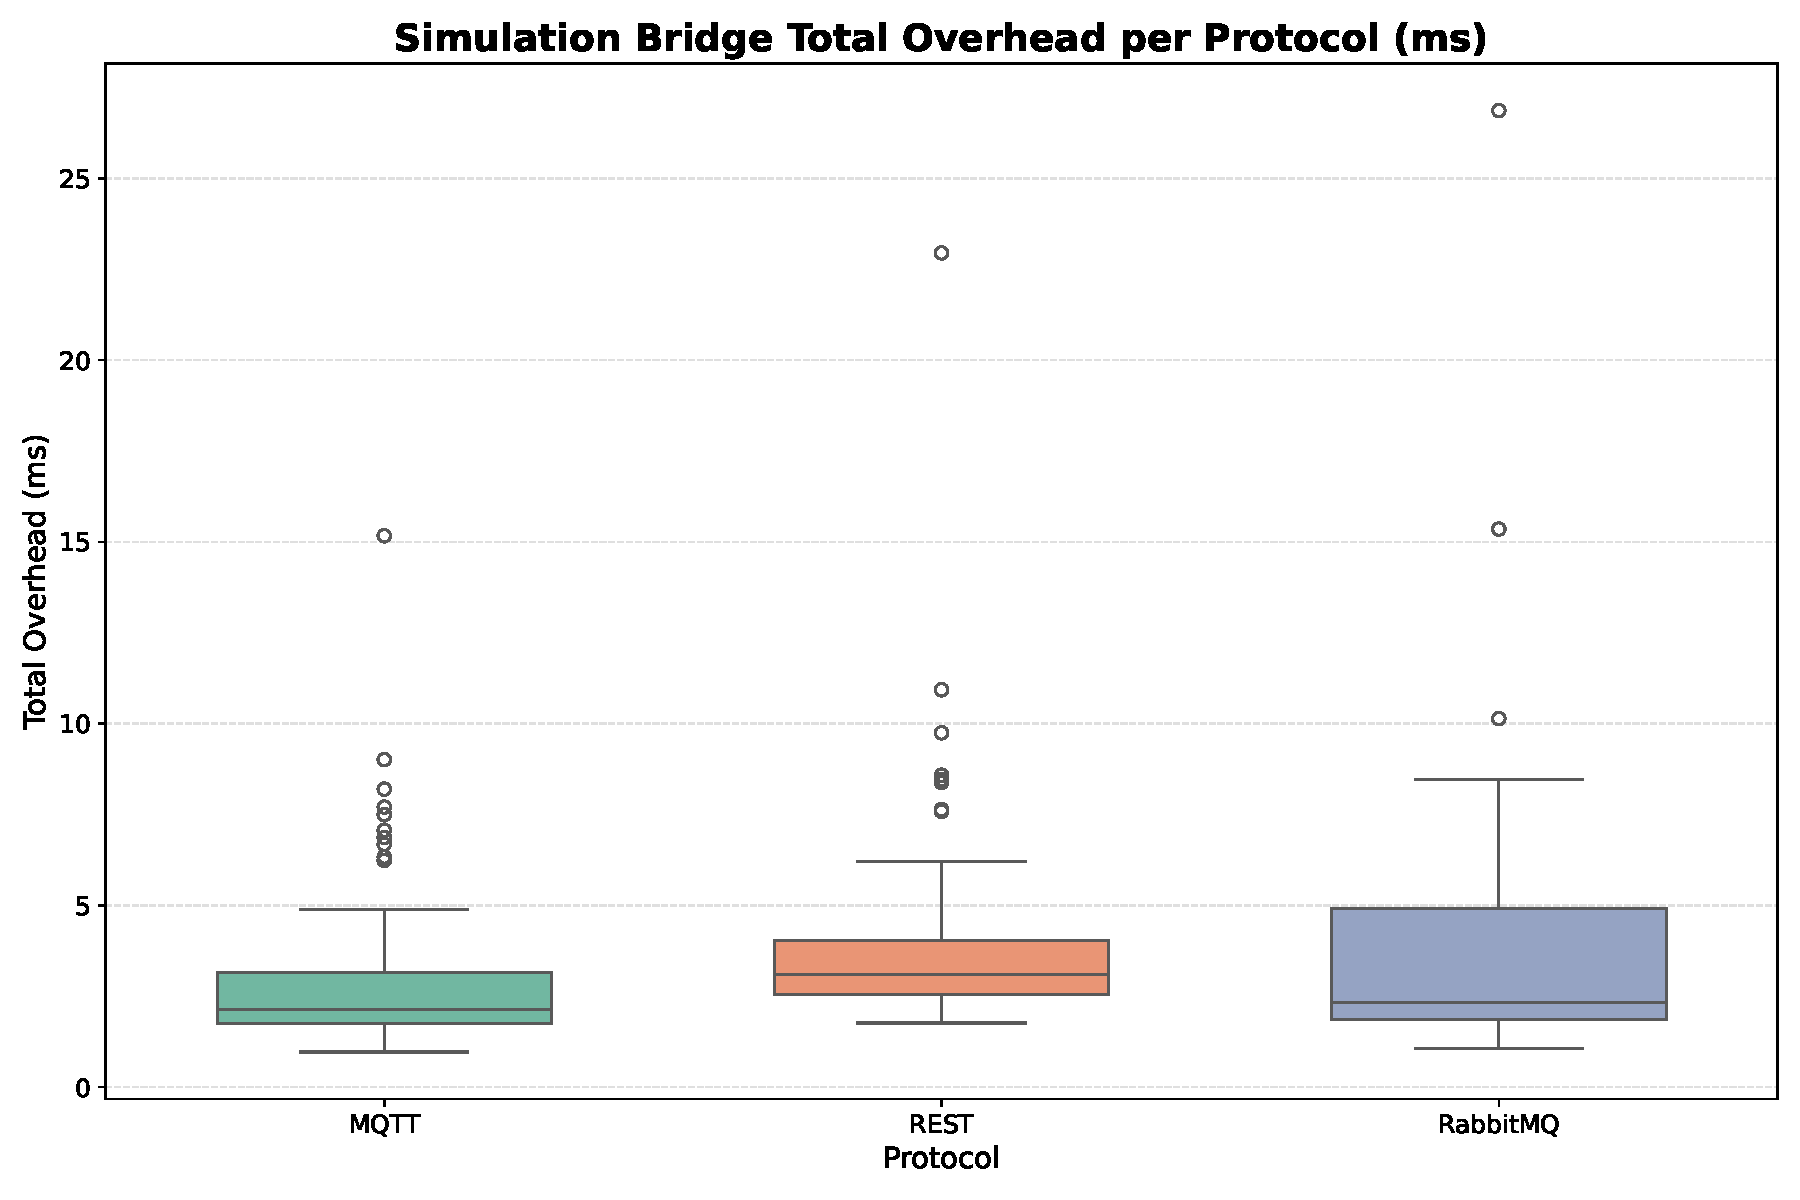
\includegraphics[width=0.9\columnwidth, trim=0in 0in 0in 0.4in, clip]{img/simulation_bridge_overhead_boxplot.pdf}
    \caption{The processing overhead in the core of the simulation bridge.}
    \label{fig:sim-bridge-overhead}
    %\vspace{-0.5cm}
\end{figure}    
\end{comment}

%%%%%%%%%%%%%%%%%%%%%%%%%%%%%%%%%%%%%%%%%%%%%%
\begin{figure*}[h]
    \centering
    \subfloat[The UR10e robotic arm in MatLab.]{
        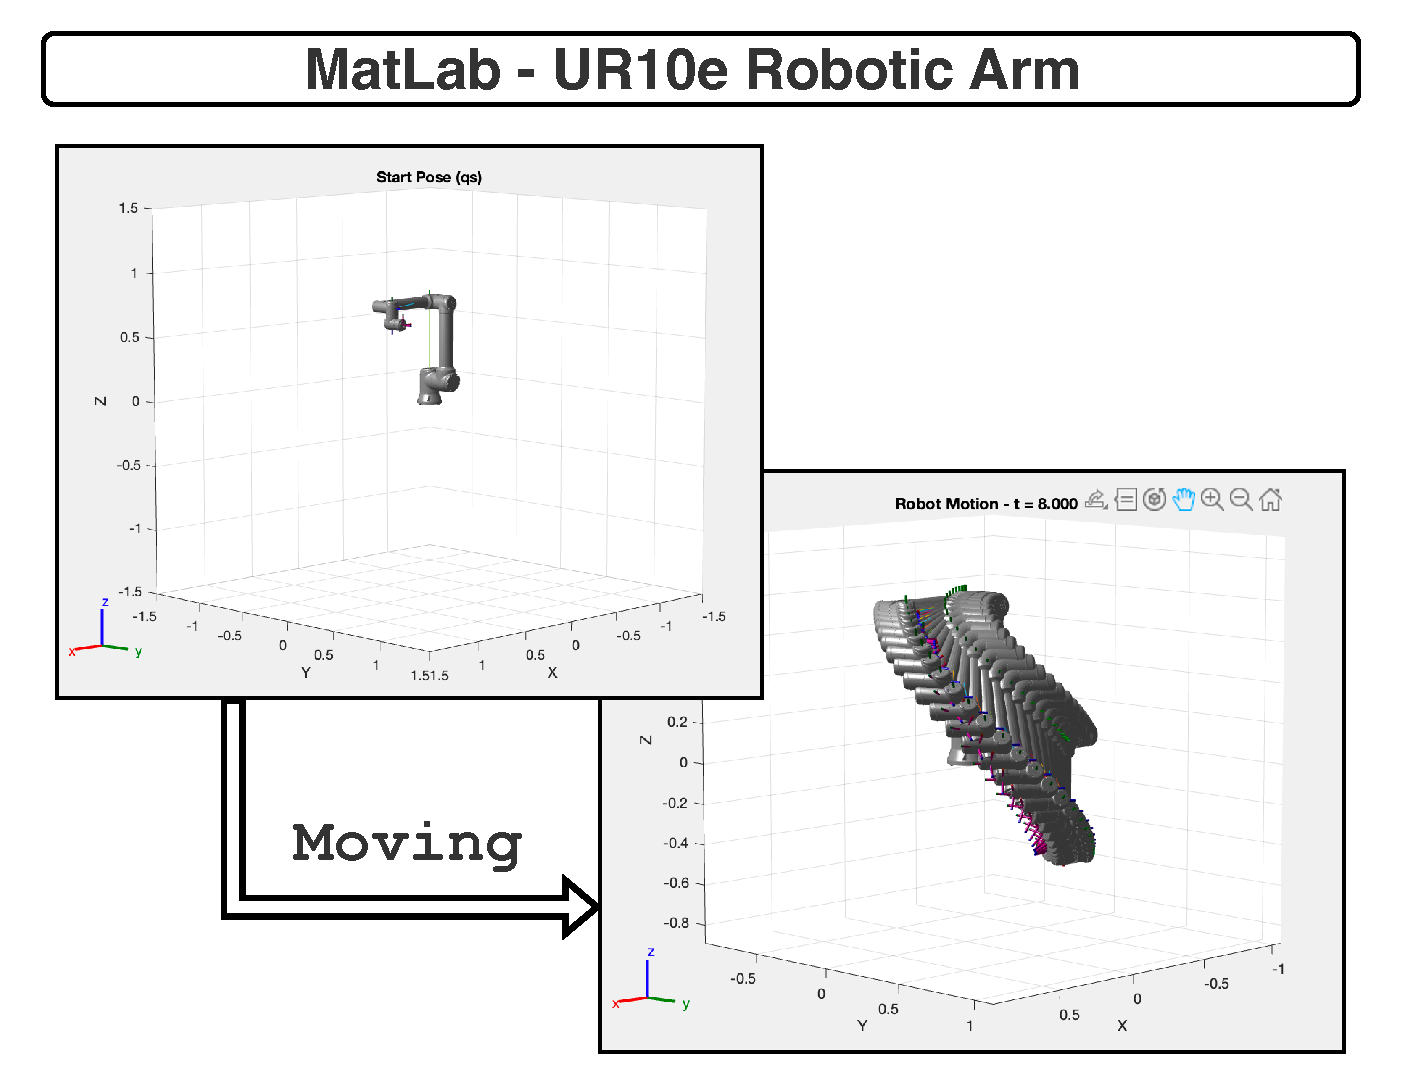
\includegraphics[width=0.465\linewidth]{img/matlab_pt.pdf}
        \label{fig:matlab_pt}
    }
    \hfill
    \subfloat[AnyLogic Microfactory simulation.]{
        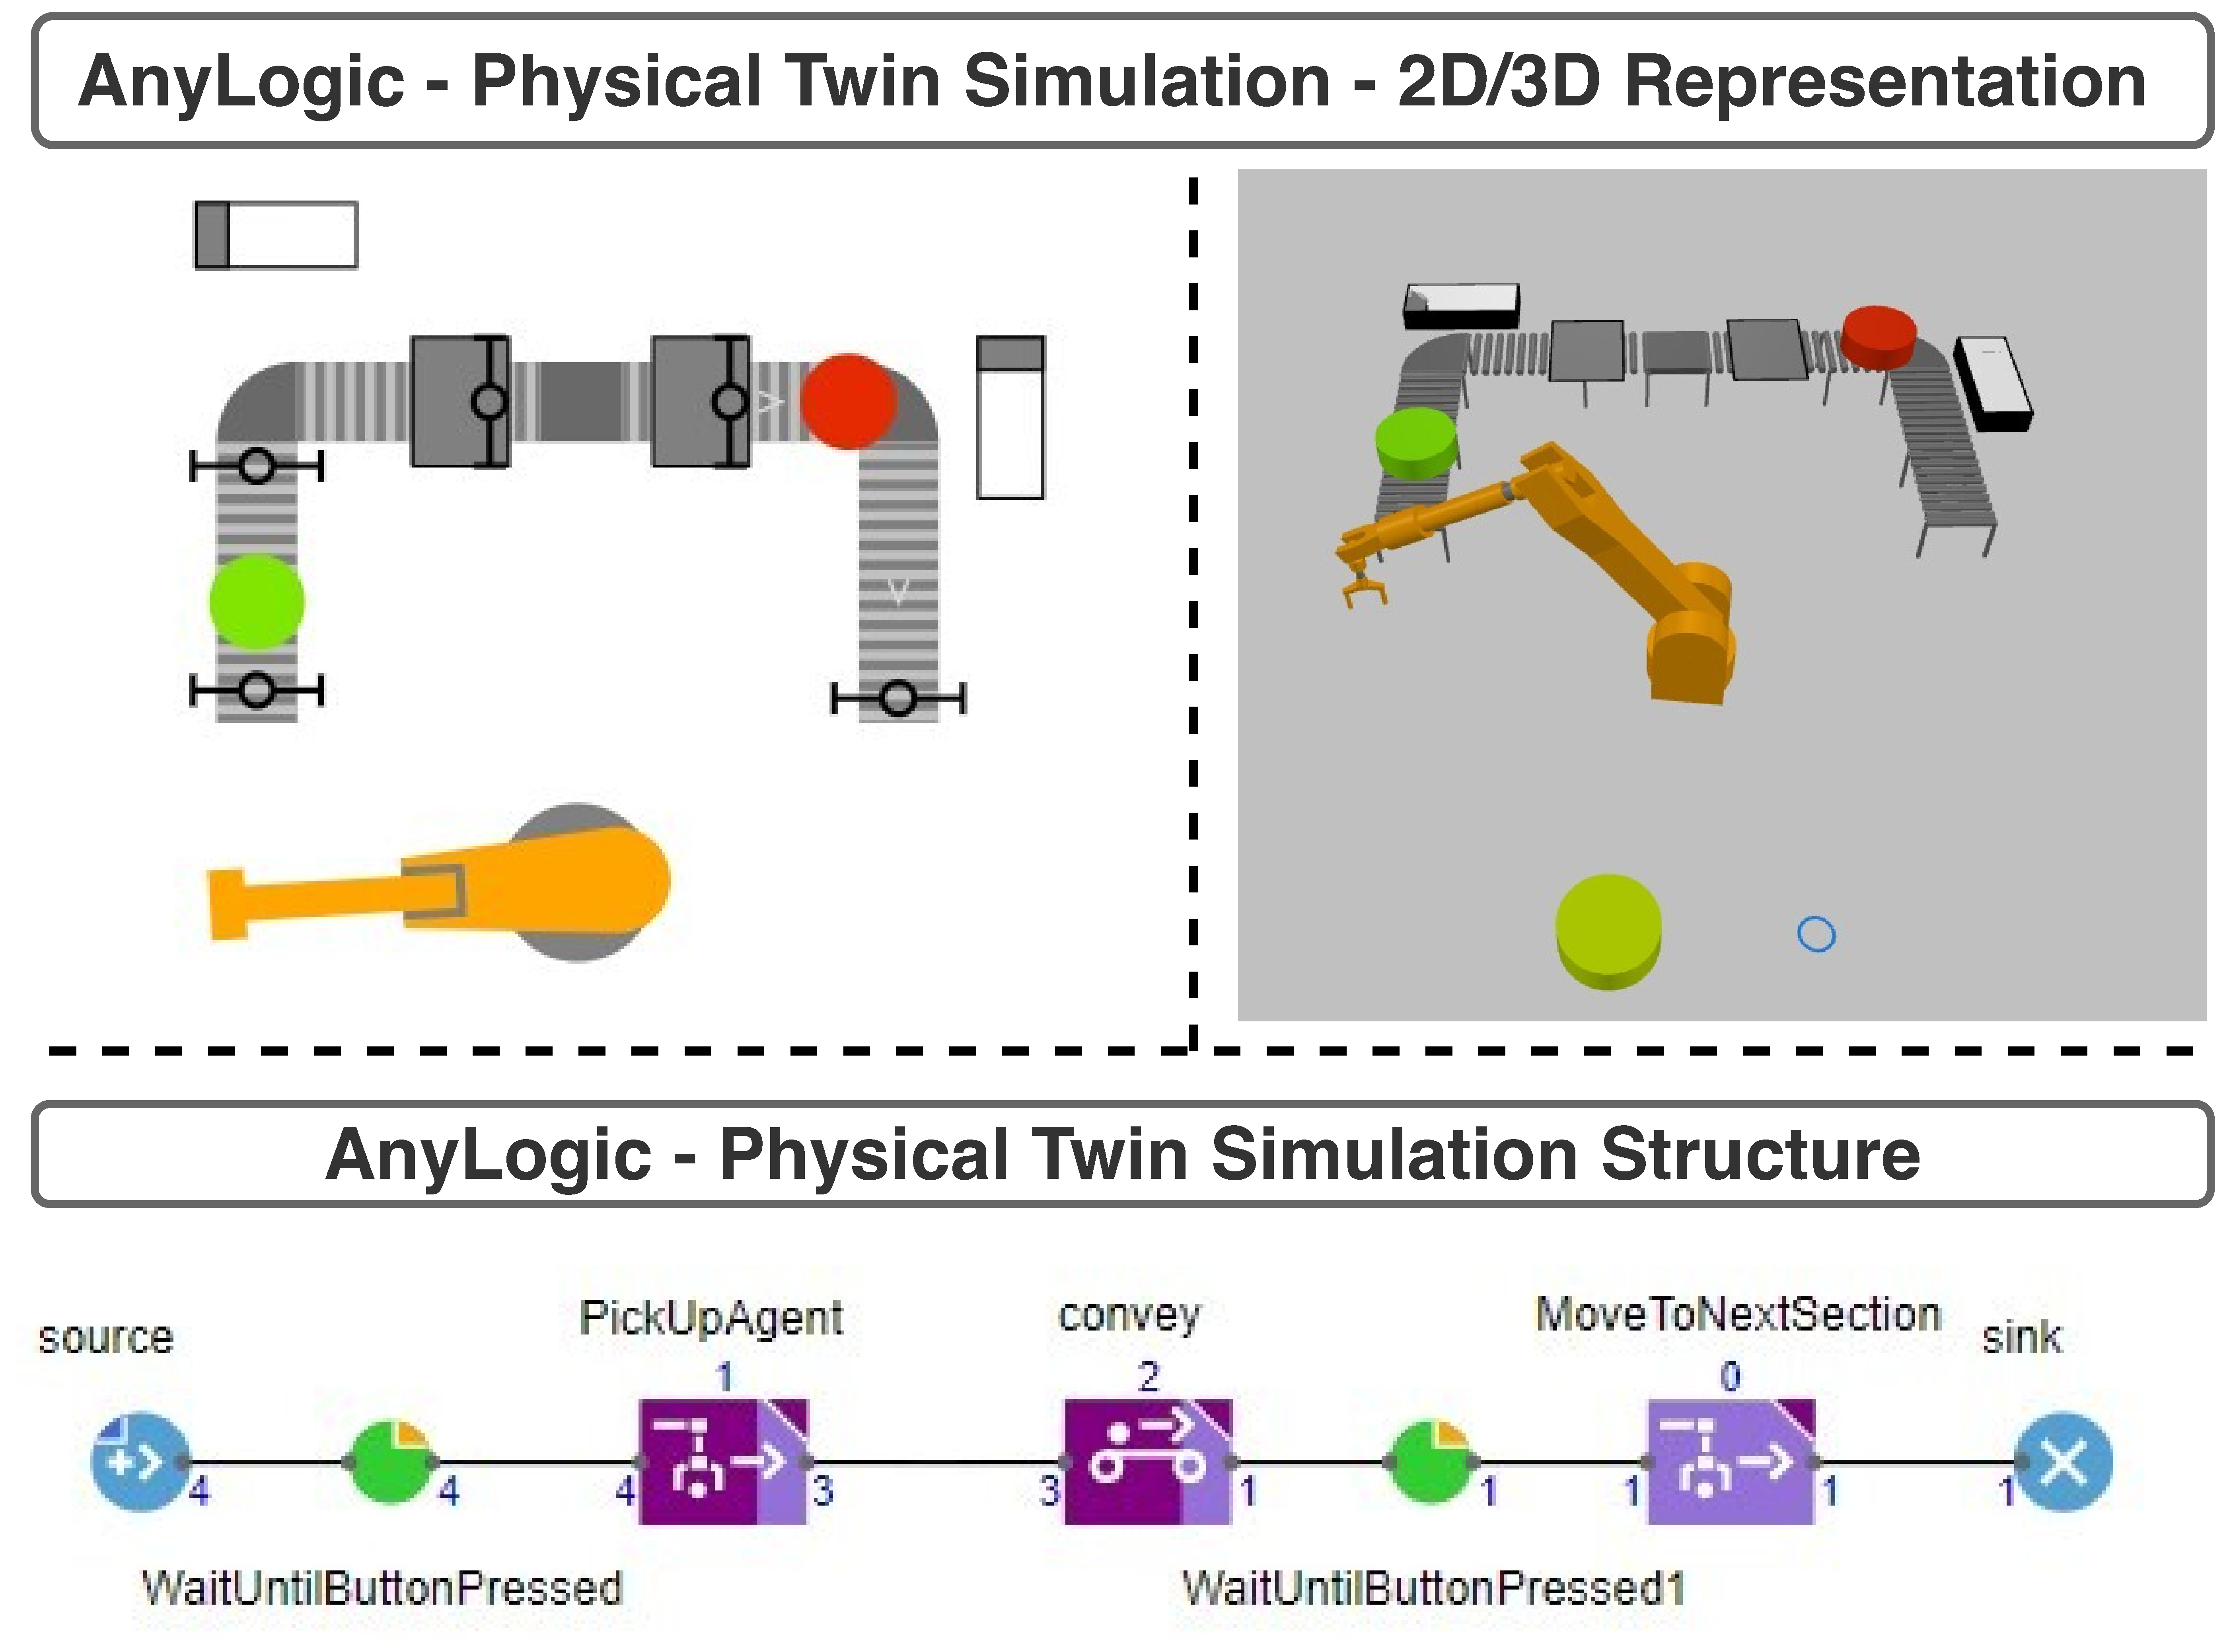
\includegraphics[width=0.48\linewidth]{img/any_logic_simple.pdf}
        \label{fig:any_logic_simple}
    }
    \caption{Simulated Physical Twins integrated with the Simulation Bridge.}
    \label{fig:physical_twin_simulations}
    \vspace{-0.5cm}
\end{figure*}
%%%%%%%%%%%%%%%%%%%%%%%%%%%%%%%%%%%%%%%%%%%%%%

\begin{table}[htbp]
\centering
\caption{Performance of DT-SB for different protocols.}
\label{tab:dt-sb_performance}
\renewcommand{\arraystretch}{1.5}
\begin{tabular}{p{0.3in}p{0.4in}p{0.3in}p{0.75in}p{0.75in}}
\hline
\textbf{Protocol} & \textbf{Overhead} & \textbf{STD} & \textbf{5\% Threshold} & \textbf{95\% Threshold} \\
\hline
MQTT & 2.47ms & 10.49ms & 1.69ms & 11.98ms \\
AMQP & 1.95ms & 0.99ms & 1.12ms & 3.69ms \\
REST & 4.63ms & 4.72ms & 2.92ms & 11.42ms \\
\hline
\end{tabular}
\vspace{-0.5cm}
\end{table}

% \begin{table}[htbp]
% \centering
% \caption{Performance comparison of DT simulation bridge for different protocol adapters. \textcolor{blue}{(The difference in values for REST/HTTP2.0 need to be explained.)}}
% \label{tab:dt-sb_performance}
% \renewcommand{\arraystretch}{1.5}
% \begin{tabular}{p{0.5in}p{0.5in}p{0.5in}p{0.5in}p{0.5in}}
% \hline
% \textbf{Protocol} & \textbf{Median Total Overhead (ms)} & \textbf{Standard Deviation (ms)} & \textbf{5\% Threshold (ms)} & \textbf{95\% Threshold (ms)} \\
% \hline
% MQTT & 2.47 & 10.49 & 1.69 & 11.98 \\
% AMQP & 1.95 & 0.99 & 1.12 & 3.69 \\
% REST (HTTP/2.0) & 4.63 & 4.72 & 2.92 & 11.42 \\
% \hline
% \end{tabular}
% \end{table}


\section{Experimental Evaluation}
\label{sec:experimental_evaluation}

To evaluate the performance of the proposed DT-SB and its integration with simulation agents, we conducted a series of experiments focusing on protocol overhead and agent-level performance on commercial computing hardware (MacBook Air Apple Silicon M2 processor and 8~GB of unified memory) with Python implementation of the proposed DT-SB \footnote{Simulation Bridge GitHub Repo: \url{https://github.com/INTO-CPS-Association/simulation-bridge}}. 

% All tests were executed on an Apple MacBook Air (2023) equipped with an Apple Silicon M2 processor and 8~GB of unified memory. MATLAB was natively installed on macOS, and Python profiling modules were used to gather performance metrics.

\subsection{Simulation Bridge Overhead}

\textbf{DT-SB Overhead}. The DT-SB was implemented to support multiple communication protocols on its north-bound interface (facing DTs), including MQTT, AMQP, and HTTP/2.0. Its south-bound interface (facing simulation agents) currently supports AMQP. We evaluated the processing time overhead introduced by the DT-SB core, explicitly excluding the contribution of individual protocol adapters.
Table \ref{tab:dt-sb_performance} shows the descriptive statistics of measured processing time overhead for MQTT, AMQP, and HTTP/2.0 protocol adapters.
These results confirm that DT-SB can reliably handle heterogeneous PAs with minimal latency in request forwarding and agent selection.
%These results indicate negligible performance differences across protocols and confirm that DT-SB can reliably handle heterogeneous DT communication channels with minimal latency in request forwarding and agent selection.

\textbf{Matlab Agent Overhead}.
% A dedicated MATLAB agent was developed to interface the DT-SB with MATLAB simulations. 
To assess the performance of the MATLAB agent independently of simulation model complexity, we used lightweight test cases to isolate the agent's intrinsic processing overhead. Each simulation request was assigned a unique \textit{Request ID}, enabling precise tracking of request-response cycles. For streaming mode experiments, different time steps were used to vary the frequency of data exchange, simulating increased communication loads.
The overhead refers to the time spent by the agent to process a simulation request, excluding MATLAB startup time and simulation runtime. This metric captures the cost of request parsing, file operations, and inter-process communication. In batch mode, the agent exhibited a mean overhead of 2.7~ms. In streaming mode, the mean overhead was 3.7~ms. Table~\ref{tab:matlab-streaming} reports the measured overhead for different streaming frequencies, showing that agent performance remains stable across varying time steps. These findings confirm that $SA_{\text{MATLAB}}$ introduces minimal latency, making it suitable for both batch and real-time streaming applications.

\begin{table}[h!]
\centering
\caption{Matlab Agent's overhead for different frequencies.}
\label{tab:matlab-streaming}
\begin{tabular}{lcccccc}
\hline
\textbf{Streaming Frequency (ms)} & 10 & 50 & 70 & 100 & 150 & 200 \\ 
\hline
\textbf{Agent Overhead (ms)} & 2.2 & 4.1 & 5.6 & 4.9 & 3.2 & 3.0 \\ 
\hline
\end{tabular}
\end{table}

\textbf{Anylogic Agent Overhead}. To evaluate the performance of the AnyLogic agent a dedicated testing campaign was conducted to measure the system’s intrinsic overhead, independently of simulation model complexity aligned with the MATLAB agent analysis. The simulation used for the experiment is shown in Figure~\ref{fig:any_logic_simple}. The AnyLogic model employed is event-based, meaning that the simulation flow is internally controlled and does not rely on a fixed time step, unlike Table~\ref{tab:matlab-streaming}, which reports the MATLAB agent’s overhead at different frequencies. To ensure comparability with previous analyses, the simulation was executed at various run-time speeds (1x, 2x, 5x, 10x, 25x, 50x). The results show an extremely low and stable average overhead, ranging from 3.4~ms to 8.6~ms across different streaming configurations, as reported in Table~\ref{tab:anylogic-streaming}. These findings confirm that $SA_{\text{AnyLogic}}$ introduces negligible latency, making it suitable for real-time streaming applications.

\begin{table}[h!]
\centering
\caption{AnyLogic Agent's overhead at different execution speeds.}
\label{tab:anylogic-streaming}
\begin{tabular}{lcccccc}
\hline
\textbf{Execution Speed} & 1x & 2x & 5x & 10x & 25x & 50x \\ 
\hline
\textbf{Agent Overhead (ms)} & 8.6 & 4.9 & 8.3 & 3.4 & 5.3 & 3.6 \\ 
\hline
\end{tabular}
\end{table}



\begin{comment}
\begin{table}[h!]
\centering
\caption{Matlab Agent's overhead for different frequencies.}
\label{tab:matlab-streaming}
\begin{tabular}{lcccccc}
\hline
\textbf{Streaming Frequency (ms)} & 10 & 50 & 70 & 100 & 150 & 200 \\ 
\hline
\textbf{Agent Overhead (ms)} & 2.2 & 4.1 & 5.6 & 4.9 & 3.2 & 3.0 \\ 
\hline
\end{tabular}
\end{table}
\end{comment}

\begin{comment}
\paragraph{Startup to Total Duration Ratio}
This metric expresses the portion of total request time spent initializing MATLAB. A high ratio indicates significant startup overhead.
\begin{center}
\begin{tabular}{|l|c|}
\hline
\textbf{Request ID} & \textbf{Startup / Total Duration Ratio} \\
\hline
streaming\_10ms  & 0.6143 \\
streaming\_50ms  & 0.5652 \\
streaming\_70ms  & 0.3907 \\
streaming\_100ms & 0.4352 \\
streaming\_150ms & 0.5369 \\
streaming\_200ms & 0.5906 \\
batch            & 0.1747 \\
\hline
\end{tabular}
\end{center}
\textbf{Mean Ratio:} \texttt{0.4725}    

\paragraph{System Resource Utilization}
The average resource usage during execution was as follows:
\begin{itemize}
    \item \textbf{Mean CPU Usage:} \texttt{94.30\%}
    \item \textbf{Mean Memory RSS:} \texttt{25.31 MB}
\end{itemize}
\end{comment}

% \begin{figure}[ht]
%     \centering
%     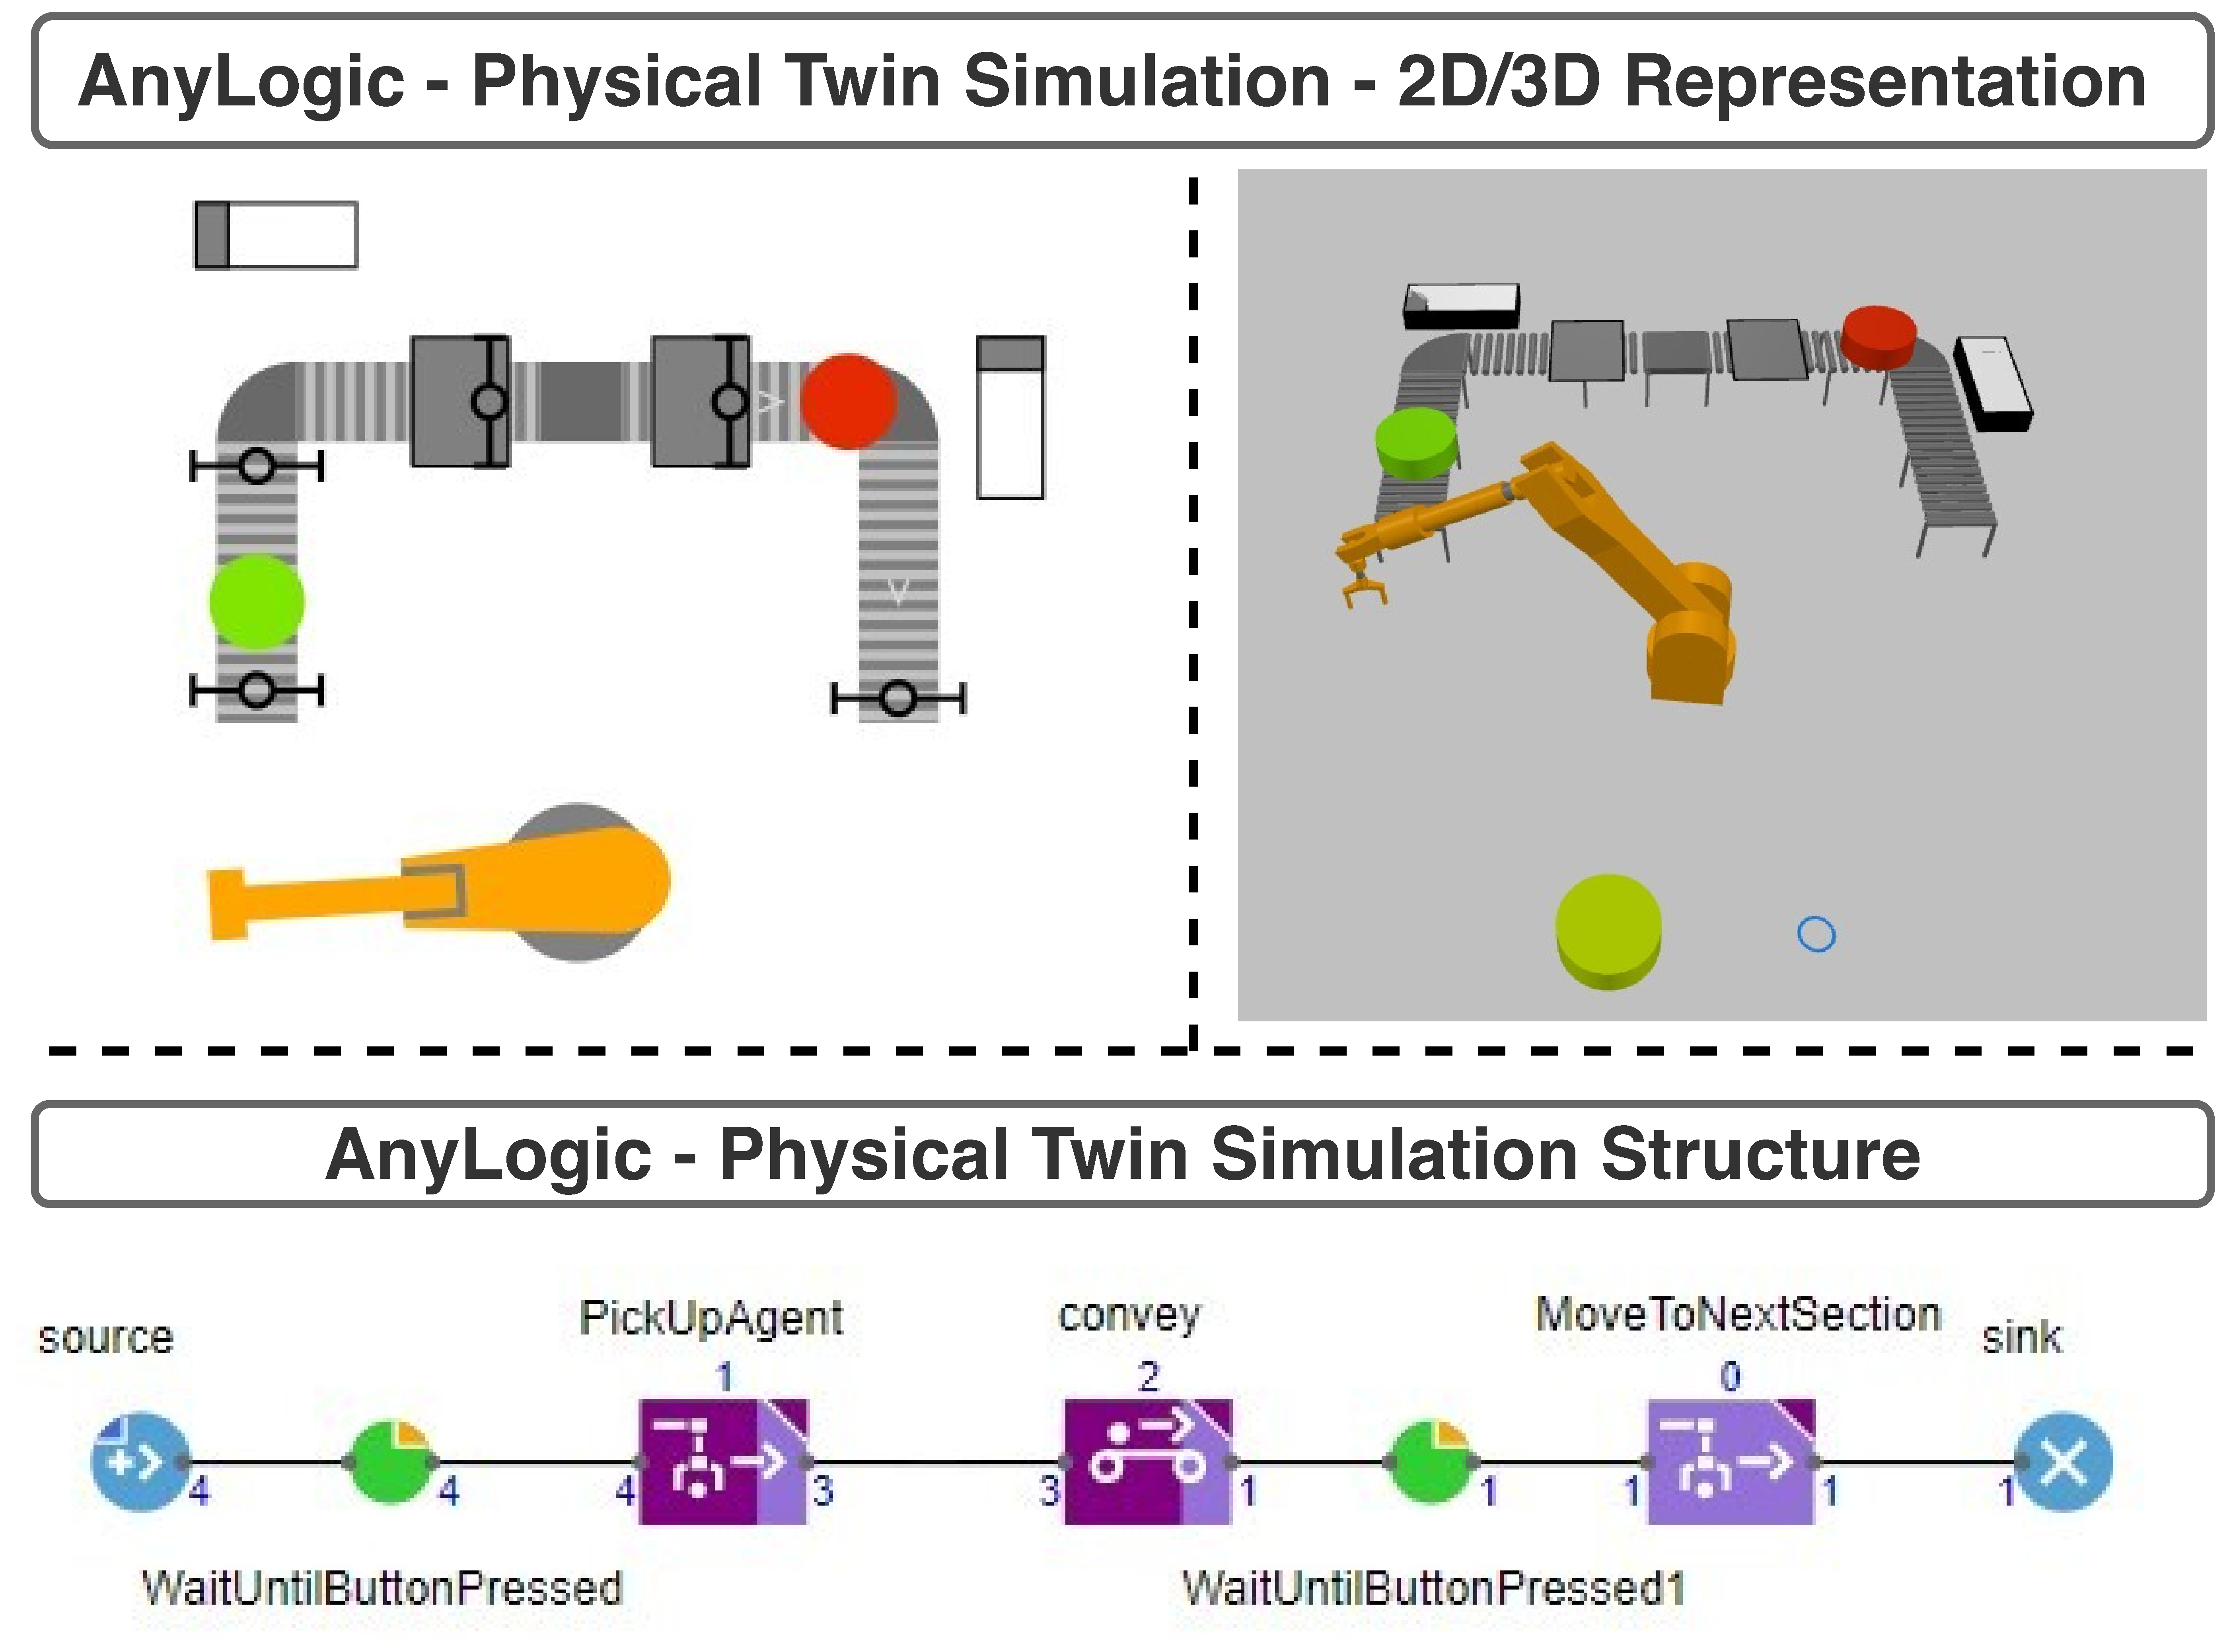
\includegraphics[width=0.9\columnwidth]{img/any_logic_simple.pdf}
%     \caption{AnyLogic PT simulation.}
%     %\Description{AnyLogic PT simulation.}
%     \label{fig:any_logic_simple}
%     \vspace{-0.5cm}
% \end{figure}

\subsection{Physical Twin Simulations}

To validate and analyze the proposed Simulation Bridge framework and the integration with DTs, two simulation environments were developed to emulate distinct aspects of the PTs behaviors: one in \textit{MATLAB/Simulink}, focusing on robotic motion control and kinematics, and one in \textit{AnyLogic}, modeling a microfactory scenario for system-level DT integration and communication assessment.

The first simulation involves a Universal Robots UR10e robotic arm executing a smooth point-to-point motion in joint space as depicted in Figure \ref{fig:matlab_pt}. The objective is to move the robot from an initial joint configuration to a target configuration within a specified time, following an optimally smooth trajectory and employing a simple closed-loop controller to track this trajectory. To ensure smooth motion, a fifth-order (quintic) polynomial trajectory was defined for each of the robot’s six joints. A quintic polynomial has six coefficients, allowing the imposition of six boundary conditions (initial and final position, velocity, and acceleration). This ensures continuity of the first and second derivatives—velocity and acceleration—throughout the entire motion.

The robotic simulation was implemented using the Robotics System Toolbox and a rigid-body model of the UR10e with gravity enabled. At each time step, the control law computed a new joint velocity command, and joint angles were updated via simple Euler integration. This iterative process continued until the planned trajectory duration elapsed. Completion was detected when the final joint configuration error dropped below a predefined negligible threshold, ensuring accurate convergence to the target configuration.

The second simulated environment was developed using the DT-SB integrated agent within \textit{AnyLogic} to support DT creation for a Microfactory scenario. The model represents an indexed production line comprising a conveyor, multiple workstations, and a robotic arm responsible for handling parts between loading and unloading areas, as illustrated in Figure~\ref{fig:any_logic_simple}. 

% The environment was built using the \textit{AnyLogic Material Handling Library}\footnote{AnyLogic Material Handling Library: \url{https://www.anylogic.com/features/libraries/material-handling-library/}}.

The two-dimensional model includes conveyors capable of reporting operational status, photocells detecting product passage, and transfer stations with custom switches emulating pusher mechanisms. Workstations are equipped with virtual actuators that communicate their operational state, while the central robot, modeled via the \textit{Robot} element, manages item positioning and state updates. Process logic is implemented using a block-diagram approach: agents are generated by a \textit{Source} block, controlled by a \textit{Hold} block linked to user interface commands, processed by a \textit{ProcessByRobot} block, transferred using a \textit{Convey} block, and finally removed by a \textit{Sink} block. 

Together, these simulation environments provided a controlled and complementary validation setup for the proposed approach. The MATLAB/Simulink model enabled low-level evaluation of motion control and trajectory tracking, while the AnyLogic microfactory scenario assessed system-level communication, synchronization, and interoperability. This combination demonstrated the framework’s flexibility in connecting diverse simulation domains within a unified DT integration architecture.

% This setup enables the DT to process data as if originating from real PTs. Communication performance was assessed by measuring the latency of bidirectional data exchange via MQTT. The average measured communication overhead from AnyLogic to the DT was \(6.5~\mathrm{ms}\) with a standard deviation of \(10~\mathrm{ms}\). Overall, the AnyLogic simulation provides a controlled and repeatable environment for DT testing, supporting experimentation on PT conditions, communication protocols, synchronization strategies, and cyber-physical system (CPS) integration.



% This use-case involves a Universal Robots UR10e robotic arm executing a smooth point-to-point motion in joint space. The objective is to move the robot from an initial joint configuration to a target configuration within a specified time, following an optimally smooth trajectory and using a simple closed-loop controller to track this trajectory.

% To ensure smooth motion, we employed a 5th-order (quintic) polynomial trajectory for each of the robot’s six joints. A quintic polynomial has six coefficients, which allows imposing six boundary conditions (start and end position, velocity, and acceleration) – exactly what is needed to guarantee continuous first and second derivatives (velocity and acceleration) throughout the motion. 

% The simulation was implemented in MATLAB/Simulink (Robotics System Toolbox) using a UR10e rigid-body model with gravity enabled. A fixed integration time-step of \(\Delta t = 5 ms\) was used to update the robot’s joint states. At each time step, the control law above was applied to compute a new joint velocity command, and the joint angles were updated as (simple Euler integration). This process was repeated until the planned trajectory time elapsed and the robot had effectively reached the goal. To determine completion, we set a very small threshold on the final error: the loop stops only once ensuring the final joint configuration is achieved with negligible error.

% The simulated environment was developed using the DT-SB integrated agent for AnyLogic to support DT creation for a microfactory scenario, featuring an indexed line with a conveyor, workstations, and a robot handling parts between loading areas, as shown in Figure~\ref{fig:any_logic_simple}.

% built with the AnyLogic Material Handling Library\footnote{AnyLogic Material Handling Library: \url{https://www.anylogic.com/features/libraries/material-handling-library/}}, 

% The two-dimensional model, includes conveyors reporting status, photocells detecting product passage, and transfer stations with custom switches emulating pushers. Workstations have virtual actuators reporting status, and the central robot, modeled via the \textit{Robot} element, manages item positioning and state updates. The simulation integrates all key entities and focuses on assessing the communication overhead of bidirectional data exchange with the DT via the DT-SB.

% Process logic uses a block diagram: agents are generated by a \textit{Source} block, controlled by a \textit{Hold} block linked to UI buttons, processed by a \textit{ProcessByRobot} block, moved via a \textit{Convey} block, and removed by a \textit{Sink} block. The DT processes data as if from real PTs. The measured communication overhead from AnyLogic to the DT via MQTT averaged $6.5\,\mathrm{ms}$ with a standard deviation of $10\,\mathrm{ms}$.

% This setup offers a controlled, repeatable environment for testing DTs, supporting experimentation with PT conditions, communication protocols, synchronization, and CPS integration strategies.


% The simulated environment was developed using the DT-SB integrated agent for AnyLogic to enable and support the creation of DTs for a microfactory scenario. This scenario features an indexed line with a conveyor, multiple workstations, and a robot that moves pieces between loading areas, as illustrated in Figure~\ref{fig:any_logic_simple}, showing both the simulation structure and the 2D/3D visualizations.

% The two-dimensional model of the indexed line was developed using elements from the AnyLogic Material Handling Library\footnote{AnyLogic Material Handling Library: \url{https://www.anylogic.com/features/libraries/material-handling-library/}}. 
% The conveyors simulate the physical transport system and report their operational status, while photocells detect and signal the passage of products at predefined positions. In the absence of dedicated pushers, transfer stations combined with a custom-designed switch emulate their functionality, sending position change messages to the Simulation Bridge. 
% The workstations are equipped with virtual actuators that report machine status and process progress. The robot at the center of the microfactory is modeled using the AnyLogic \textit{Robot} element, which handles item positioning and transmits state updates, such as item pick-up events. 
% The target simulation integrated all core production entities---the conveyor, robotic arm, workstations, photocells, and product flow---and focused on evaluating the communication overhead of bidirectional data exchange between the DT and the simulation environment through the DT Simulation Bridge.

% The process logic is implemented as a block diagram. Simulation agents are generated by a \textit{Source} block, controlled by a \textit{Hold} block linked to UI buttons that govern robot operation. Items are processed by a \textit{ProcessByRobot} block defining pick-and-place tasks, moved along conveyor paths via a \textit{Convey} block, and finally removed by a \textit{Sink} block. 
% In this setup, the DT processes data as if it were sent from real Physical Twins, although these are simulated. The measured communication overhead, from the AnyLogic simulation environment to the DT via MQTT, resulted in an average delay of approximately $6.5 \,\mathrm{ms}$, with a standard deviation of about $10 \,\mathrm{ms}$.

% This integrated industrial simulation, combined with the DT-SB, provides a controlled, repeatable environment for developing and testing DTs. It supports experimentation with different PT conditions, communication protocols, synchronization mechanisms, and integration strategies for physical and CPSs.



\section{Conclusion}
\label{sec:conclusion}

In this paper, we tackled the integration of heterogeneous simulations with DTs via a general-purpose middleware framework. We analyzed key interaction patterns---\emph{batch}, \emph{streaming}, and \emph{PT simulation}---supporting various DT lifecycle use cases. We proposed the \emph{DT Simulation Bridge (DT-SB)} architecture and a lightweight protocol that ensures a uniform interface between DTs and diverse simulation environments. The DT-SB enables data translation, protocol adaptation, and interoperability across platforms. We validated our solution through two case studies: \textit{(i)} MATLAB-based streaming performance evaluation; and \textit{(ii)} AnyLogic-based PT simulation of a cyber-physical scenario. Future work will focus on classifying integration patterns, extending to co-simulation and hybrid setups, refining synchronization, and exploring adaptive orchestration in distributed environments.

\bibliographystyle{ACM-Reference-Format}
\bibliography{bibliography}


\end{document}
